% %%%%%%%%%%%%%%%%%%%%%%%%%%%%%%%%%%%%%%%%%%%%%%%%%%%%%%%%%%%%%%%%%%%%%%
% Dummy Chapter:
% %%%%%%%%%%%%%%%%%%%%%%%%%%%%%%%%%%%%%%%%%%%%%%%%%%%%%%%%%%%%%%%%%%%%%%

% %%%%%%%%%%%%%%%%%%%%%%%%%%%%%%%%%%%%%%%%%%%%%%%%%%%%%%%%%%%%%%%%%%%%%%
% The Introduction:
% %%%%%%%%%%%%%%%%%%%%%%%%%%%%%%%%%%%%%%%%%%%%%%%%%%%%%%%%%%%%%%%%%%%%%%
\fancychapter{Minimal models of electron correlations in energy bands}
\label{cap:hubbard}

\slshape

We start with an overview of the Hubbard model and in the following chapters we provide details on how to simulate it numerically using Quantum Monte Carlo. In particular, we discuss the original motivation provided by Hubbard to introduce the model and show how its Hamiltonian arises as an approximate representation of the Coulomb repulsion between electrons in a solid. Then, we present exact solutions for particular limiting cases, which will be used to crosscheck our simulations. In particular, we show that, in the limit where the interaction is large, the effective Hamiltonian at half filling corresponds to an atomic Heisenberg model defined in the appropriate Hilbert space with one electron per site.

\normalfont

\section{Introduction}\label{sec:intro}

The Hubbard model appeared in 1963 as one of the first attempts to include electron correlation effects in a quantum mechanical description of a solid \cite{Hubbard1963}. Originally, it was introduced to explain the behavior of the electrons occupying the narrow, partially filled $d-$bands of transition metals. Correlation phenomena in these bands lead to a behavior reminiscent of the atomic picture of a solid. In fact, the Hubbard model may simply be regarded as a minimal model of interacting electrons in an energy band of a solid. We have come a long way since the introduction of the Hubbard model and it is now as paradigm-defining in many-body theory as the Ising model in statistical physics\cite{Mahan2000}.

\begin{figure}[H]
	\centering
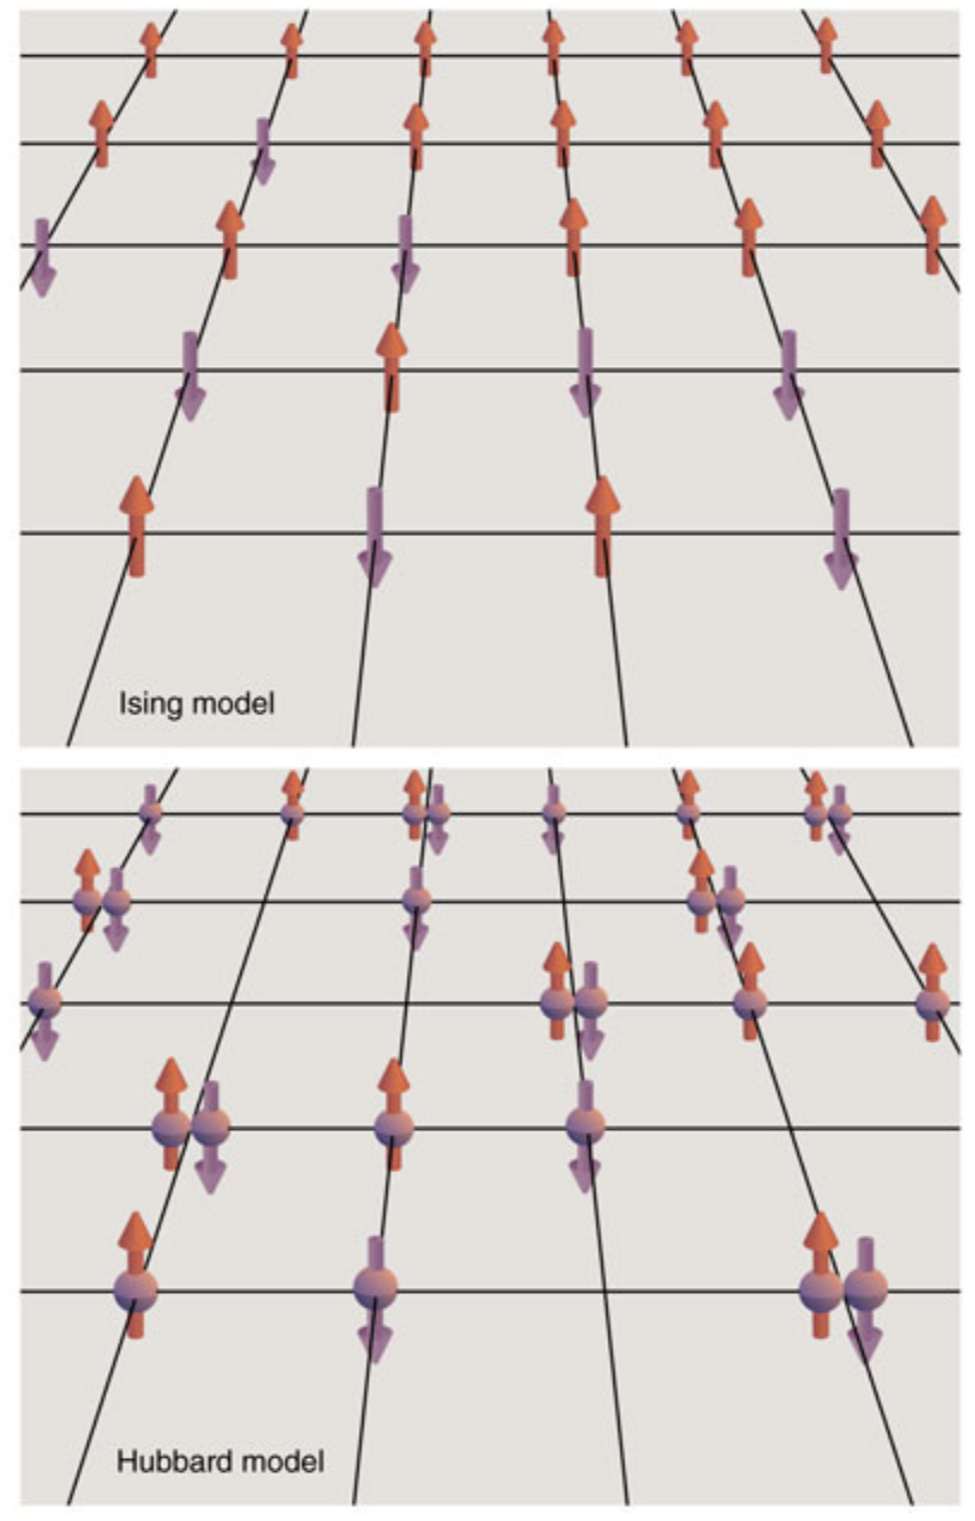
\includegraphics[width=0.5\linewidth]{Figures/3.HubbardModel/isingVsHubbard}
	\caption[Graphical comparison between the Ising and the Hubbard model.]{hi}
	\label{fig:dummyfigure1}
\end{figure}

Unlike the Ising model, where either an up or a down spin live at each site, in the Hubbard model each site can have either no spin, either an up or a down spin, or both.

When Hubbard's seminal paper came out, it followed a trend that arose in the 1950's when people were working on a theory of correlation effects in the free electron gas \cite{Bohm1953, Gell-Mann1957, Sawada1957, Hubbard1957, Hubbard1958, Nozieres1958}. Hubbard devised a simple model for the seemingly intractable problem of interacting electrons in a band. His work explained qualitatively some properties of transition and rare-earth metals in which electron correlations are non negligible. It turns out that the mathematical formulation of the interaction problem for correlated electrons in a band is not prohibitively complicated, and is relatively amenable to both analytical and numerical computations after some reasonable approximations are introduced. Notably, the model is particularly adapted to computer simulations because of its simple approximate Hamiltonian. Moreover, it has been shown to be very relevant in the description of Mott insulators, and high $T_c$ superconductors. In fact, the Hubbard model has found many applications, describing successfully a variety of quantum systems\cite{Editorial2013}; nonetheless, even the simplified picture it offers is in general difficult to approach analytically. There exists an exact solution in one dimension via Bethe ansatz\cite{Lieb1968}, but the more general higher dimensional case is often solved numerically.  Moreover, the solution obtained analytically is not very transparent, and it is hard to extract physical interpretations. An example of particular relevance for the work of this thesis is the study carried out by Hirsch \cite{Hirsch1985}. In the following chapters, we will discuss how to simulate the Hubbard model using a numerical approach that is based on this seminal paper, and in many ways follows the ideas introduced in it.


\section{Hubbard model}\label{sec:hubbardModel}

The nearly free electron gas models the conduction bands of metals and alloys fairly accurately.
The high mobility of the electrons compared to the ions justifies two equivalent approximations, both giving essentially the same results \cite{ashcroft_solid_1976}.
The first idea is to treat the periodic potential created by the \emph{virtually} fixed ions (compared to the electrons) as a perturbation on the free electron gas.
Equivalently, we may imagine the system as a collection of tightly bond atoms, in which the electrons in the higher energy band hop from atom to atom.
Both these approaches lead to band theory, a framework which allows us to predict whether a material is a conductor or a insulator.
From the tight binding point of view, the effect of the electron mobility is the broadening of the atomic energy levels: the electrons in the solid occupy energy bands, rather than levels.
The partially filled band of highest energy is called the conduction band, since it is the band occupied by conduction electrons hopping from atom to atom.
However, in transition metal and rare-earths, as in some compounds containing these elements, apart from the conduction bands there are partially filled bands: $d-$ or $f-$bands.
The partial filling of these bands and the electron correlations within them are responsible for the characteristic properties of these solids.
Some of these properties are not explained by band theory, namely the Mott metal-insulator transition \cite{h_de_boer_semiconductors_1937, mott_discussion_1937, mott_basis_1949}.

\subsection{Electron correlations in narrow $d-$bands}

First, note that the effects of correlations cannot possibly be the same in narrow energy bands and in the free electron gas.
To see this, we may simply recall the shape of a $d-$wave function.
In a $d-$orbital, the electron charge density is concentrated near the nucleus.
In a solid, the electronic charge density should then also be concentrated near the nuclei, as long as the atomic description is useful, even if not completely correct\footnote{The electronic charge density is, of course, not actually defined in terms of a squared norm of the $d-$wave function for a narrow band. There is some broadening of the corresponding atomic energy level, and the wave function describing an electron is a Bloch wave function. Since the band is narrow, we assume that the atomic wave function description is still somewhat useful in a given range and we use it to provide a heuristic motivation for the non validity of the free electron assumption.}.
It is much smaller between atoms so that electrons do seem to belong to individual atoms in some sense.
For a $d-$band, we assume that the case should not be so different since the band is narrow.
The fact that we may speak with some meaning of an electron belonging to a particular atom motivates a description from which the atomic characteristics of the solid emerge, in spite of the fact that the bandwidth of a $d-$band is still appreciable.
The point is that electrons in $d-$bands are certainly not well described by a free electron gas, which cannot possibly account for atomic-like behavior.

\begin{figure}[H]\label{fig:hydrogenWF}
\centering
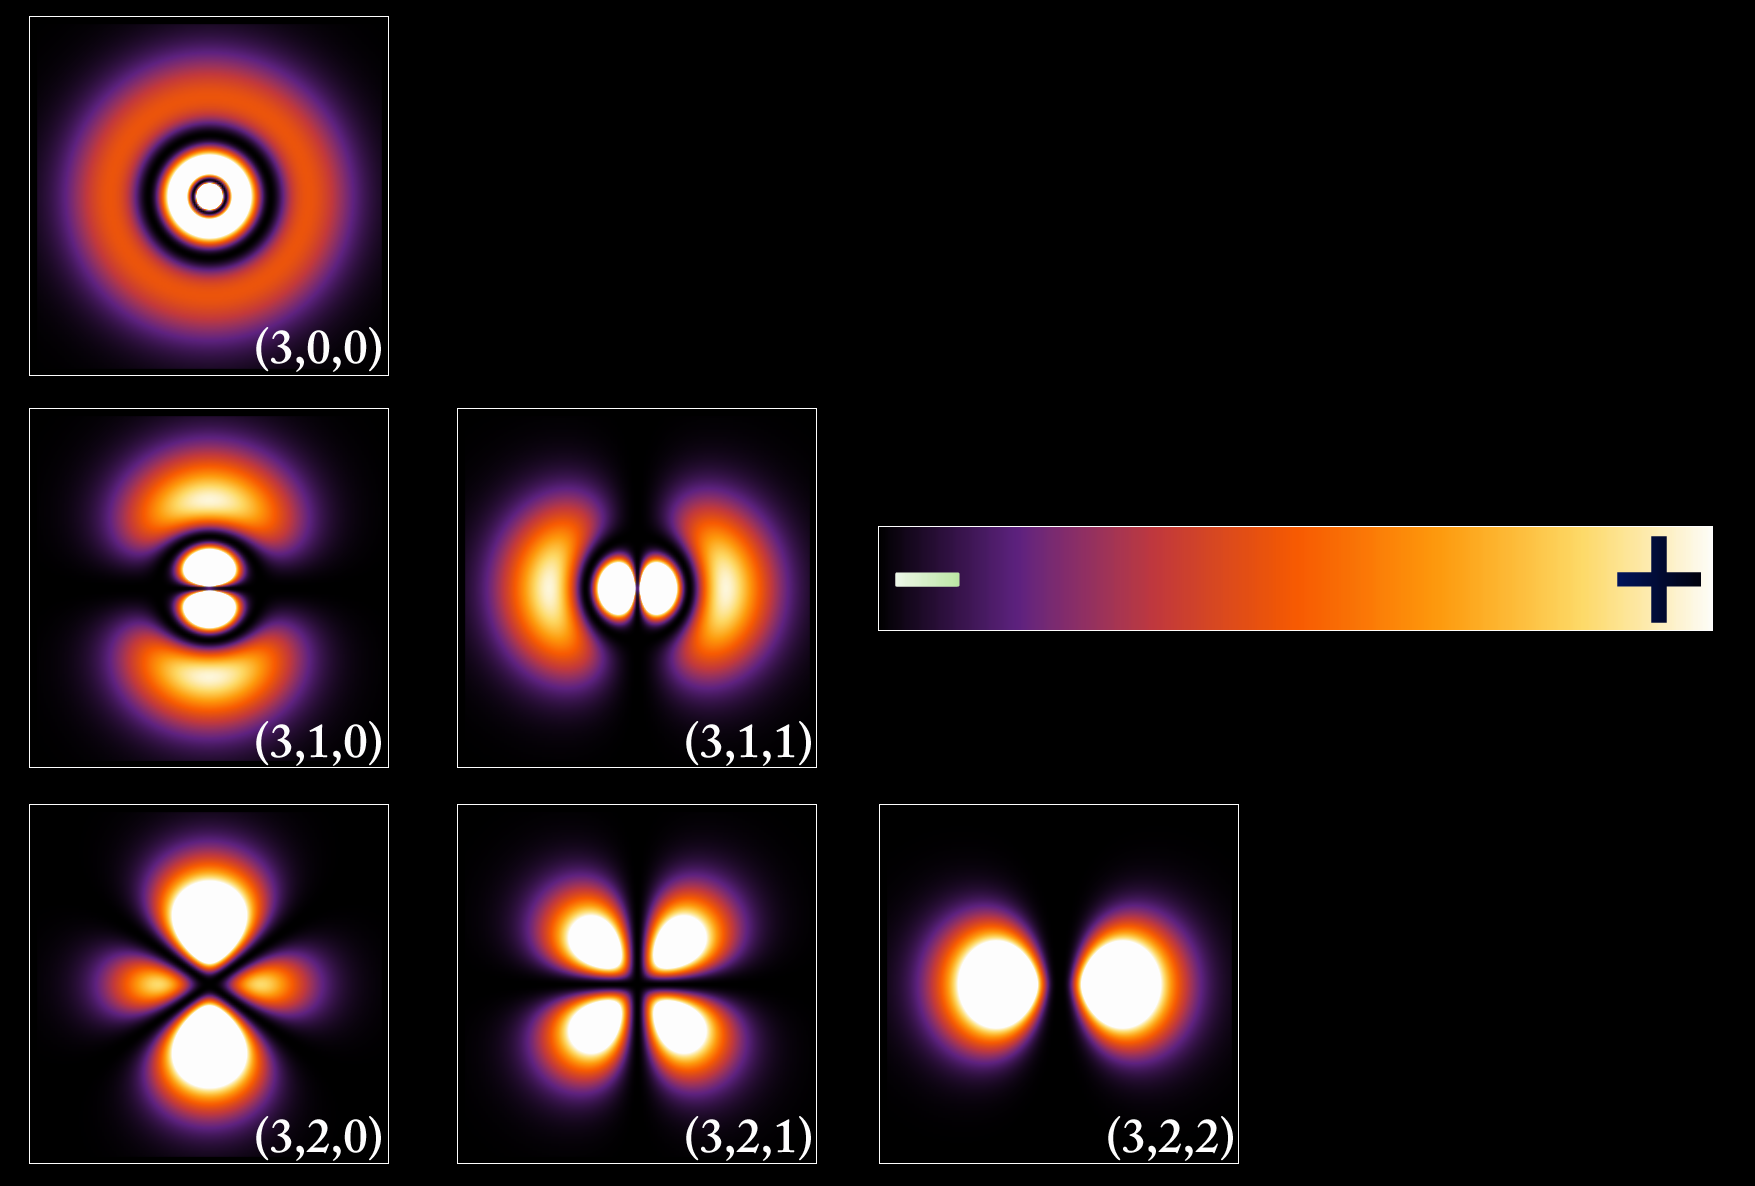
\includegraphics[width = 8.2cm]{Hubbard/Hydrogen_Density_Plots.png}
\caption[Hydrogen atomic wave functions.]{Probability density plots for different hydrogen orbital wave functions corresponding to quantum numbers $(n, l, m)$ for $n = 3$.
d-wave functions correspond to $l=2$. Note that the probability density is always higher in a region near the nucleus, and has a complicated shape, which will lead to a non-uniform distribution of electronic charge, as opposed to the case of the free electron gas. (adapted from \cite{hydrogen})}
\end{figure}

Experimentally, $d-$electrons of transition metals show a hybrid behavior: sometimes they are accurately described by an ordinary band model, but there are occasions in which the atomic model is better.
For example, we see spin wave phenomena in ferromagnetic transition metals, and the susceptibilities of some of these metals depend strongly on temperature.
This is characteristic of an atomic (Heisenberg) model.
On the other hand, the $d-$electrons contribute significantly to the low temperature specific heat and sometimes the magnetic moments per atom of some transition metal ferromagnets are not integer multiples of the Bohr magneton.
This is characteristic of band theory\footnote{Think, for example, of a tight binding model. Electrons hop from atom to atom, and in general the spin of each atom depends on the particular electrons \say{belonging} to it at a given time. If we take an average of the total spin of each atom, we will in general not necessarily obtain an integer multiple of the Bohr magneton. If we simply had a collection of atoms, Hund's rule would apply, and each atom would have its spin aligned in a given direction. The average spin would then tend to be an integer multiple of the Bohr magneton.}.
Our theory of correlations should describe this balance between band-like and atomic-like behavior.

The atomic picture of a solid consists of an electron gas where ions are immersed.
The ions then interact in much the same way as they do in salts.
This extreme scenario is surely not even close to the true state of affairs since the number of $d-$electrons per atom is in general not an integer.
This motivates us to introduce a less restrictive model, which is not too far from the atomic model.
We shall assume that while $d-$electrons still have some band motion, they are strongly correlated with each other so that the metal retains some atomic-like behavior.
The correlations between electrons on different atoms are likely much weaker and we neglect them.

Let us now look at an example of the aforementioned circumstance.
Take a partially filled $d-$band of non-interacting electrons.
The spin of any given atom in the solid is just the total spin of all electrons on that atom.
It fluctuates both in magnitude and in direction, with a characteristic time that depends on how frequently $d-$electrons hop (in the loose quantum mechanical sense).
We can estimate the time interval between $d-$electron hopping events between atoms as a being of the order $\hbar / \Delta$, where $\Delta$ is the $d-$electron bandwidth.
The spin can thus be thought of as being associated to each individual (and constantly hopping) $d-$electron.

How do the electron interactions affect this picture?
We start by recalling Hund's rule: the nature of the  interactions between atoms leads to an alignment of the spins on each atom.
Since the atomic picture seems to prevail in our metal, we have reason to expect a similar effect to occur.
An atom with a total spin in some direction at a given time will tend to attract electrons with the spin on that direction and repel those with opposite spin.
This mechanism makes it unlikely for the spin of an atom to change much over time.

If the interactions between atoms are strong enough, the correlations become considerable, and to state it more precisely, the total spin of an atom will persist for a time that is long compared with the $d-$electron hopping time.
Note that it is not the localization of the electrons that causes the spin state of the atom to persist.
The specific electrons belonging to a given atom change all the time as long as their spin is consistent with the total spin requirement imposed by Hund's rule.
For strong enough correlations, we may think of the spin as being associated to each atom, which opens up the possibility to describe the system using an atomic (Heisenberg) model, as we shall see later.

A theory of electron correlations in a narrow energy band should reduce to an atomic model in the appropriate limit, for example atoms that are so far apart on a lattice that they interact only very weakly.
Although we always keep in mind that we are focusing on $d-$electrons, we shall consider $s-$electrons in what follows for the sake of simplicity.
The important conclusions will not differ significantly.
We will use the "atomicity" of the electronic distribution to introduce an approximate representation of the electron interaction.
It turns out that this representation is mathematically much simpler to handle than the Coulomb interaction itself.

In short, our picture is the following: electrons hop rapidly from atom to atom in a band-like fashion, but their motion is correlated in such a way that atomic characteristics emerge.
The extent of atomic behavior depends, of course, on the strength of the interaction.

\subsection{Hubbard Hamiltonian}\label{hubbardHamiltonian}

Imagine a hypothetical partially filled narrow $s-$band with $n$ electrons per atom.
Suppose you have obtained Bloch wave functions $\psi_{\bm k}$ corresponding to energies $\varepsilon_{\bm k}$ by solving the Schr\"odinger equation for some spin-independent mean field Hartree-Fock potential that accounts for the average interaction of the $s-$band electrons with electrons on other bands, and the interaction with the other $s-$electrons.
The electrons on the band evolve according to the Hamiltonian:

\begin{equation}\label{eq:startingHamiltonian}
\begin{split}
&\mathcal{H} = \sum_{\bm k \sigma} \varepsilon_{\bm k} c_{\bm k \sigma}^\dagger c_{\bm k \sigma} + \frac{1}{2} \sum_{ \substack{\bm k_1 \bm k_2 \\ \bm k_1' \bm k_2' \\ \sigma_1 \sigma_2 } } \left\langle \bm k_1 \bm k_2 \bigg| \frac{e^2}{r} \bigg| \bm k_1' \bm k_2' \right\rangle 
 c_{\bm k_1 \sigma_1}^\dagger c_{\bm k_2 \sigma_2}^\dagger c_{\bm k_2' \sigma_2} c_{\bm k_1' \sigma_1} \\
 &- \sum_{ \substack{\bm k \bm k' \\ \sigma} } \bigg[ 2 \left\langle \bm k \bm k' \bigg| \frac{e^2}{r} \bigg| \bm k \bm k' \right\rangle - \left\langle \bm k \bm k' \bigg| \frac{e^2}{r} \bigg| \bm k' \bm k \right\rangle \bigg] \nu_{\bm k'} c_{\bm k \sigma}^\dagger c_{\bm k \sigma} ,
\end{split}
\end{equation}
where the $\bm k-$sums run over the first Brillouin zone.

The integrals are defined by

\begin{equation}\label{eq:integrals}
\left\langle \bm k_1 \bm k_2 \bigg| \frac{e^2}{r} \bigg| \bm k_1' \bm k_2' \right\rangle \equiv V^{\bm k_1 \bm k_2}_{\bm k_1' \bm k_2'}  =  e^2 \int \frac{\psi_{\bm k_1}^\star (\bm x) \psi_{\bm k_1'} (\bm x) \psi_{\bm k_2}^\star (\bm x') \psi_{\bm k_2'}(\bm x') }{| \bm x - \bm x' |} d\bm x d\bm x'
\end{equation}

The first term represents the band energies of the electrons and the second term represents the interactions among them.
The last term subtracts the potential energy of the electrons in the part of the Hartree-Fock field due to the electrons of the $s-$band itself.
This term ensures that we do not overestimate the magnitude of the interactions between the electrons of the band: the Hartree-Fock field that specifies $\varepsilon_{\bm k}$ is computed taking into account these interactions, so if we didn't subtract the last term, we would count the energy of these interactions twice since they reappear in the second term.
Furthermore, we assume that up and down spins are occupied equally, and $\nu_{\bm k}$ are the occupation numbers of the states of the band in the Hartree-Fock calculation. 

The term that we subtract in equation ($\ref{eq:startingHamiltonian}$) corresponds to the part of the interaction term which is already accounted for by the first diagonal mean field term.
Thus, it corresponds to the mean field expansion of the interaction term (i.e. the second term), which is generically written

\begin{equation}\label{eq:vInt}
V_{\text{int}} = \frac{1}{2} V^{\nu\mu}_{\nu'\mu'} c_\nu^\dagger c_\mu^\dagger c_{\mu'} c_{\nu'} ,
\end{equation}
where the summation over repeated indices is implied. 

In appendix \ref{ap:hartree-fock}, we obtain the mean field form of $V_{\text{int}}$ in the Hartree-Fock approximation.

Now consider the Wannier functions

\begin{equation}
\phi(\bm x) = N^{-1/2} \sum_{\bm k} \psi_{\bm k} (\bm x) , 
\end{equation}
where $N$ is the number of atoms.

We may write $\psi_{\bm k}$ as a combination of Wannier functions localized at each atom.

\begin{equation}
\psi_{\bm k} (\bm x) = N^{-1/2} \sum_i e^{i \bm k \cdot \bm R_i} \phi (\bm x - \bm R_i) ,
\end{equation}
where the sum runs over all atomic positions $\bm R_i$. 

Introducting the annihilation (creation) operators of an electron of spin $\sigma$ in the orbital state $\phi (\bm x - \bm R_i)$ (at site $i$), $c_{i\sigma}^{(\dagger)}$, we may write

\begin{equation}
c_{\bm k \sigma}^{(\dagger)} = N^{-1/2} \sum_i e^{i \bm k \cdot \bm R_i} c_{i\sigma}^{(\dagger)}
\end{equation}

Thus, the Hamiltonian becomes 

\begin{equation}
\begin{split}
&\mathcal{H} = \sum_{\substack{ i j \\ \sigma} } K_{ij} c_{i \sigma}^\dagger c_{j \sigma} + \frac{1}{2} \sum_{\substack{i j k l \\ \sigma \sigma'} }\left\langle i j \bigg| \frac{e^2}{r} \bigg| k l \right\rangle 
 c_{i \sigma}^\dagger c_{j \sigma'}^\dagger c_{l \sigma'} c_{ k \sigma} \\
 &- \sum_{\substack{ijkl \\ \sigma }} \bigg[ 2 \left\langle i j \bigg| \frac{e^2}{r} \bigg| k l \right\rangle - \left\langle i j \bigg| \frac{e^2}{r} \bigg| l k \right\rangle \bigg] \nu_{j l} c_{i \sigma}^\dagger c_{ k \sigma} ,
\end{split}
\end{equation}
where

\begin{equation}\label{eq:hopping_matrix}
K_{ij} = N^{-1} \sum_{\bm k} \varepsilon_{\bm k} e^{i \bm k \cdot ( \bm R_i - \bm R_j )},
\end{equation}
and

\begin{equation}
\nu_{j l} = N^{-1} \sum_{\bm k} e^{i \bm k \cdot ( \bm R_j - \bm R_l) }
\end{equation}

Now comes the crucial approximation.
For a narrow energy band, the Wannier functions $\phi$ nearly coincide with atomic $s-$functions.
For small bandwidth, these $s-$functions form an atomic shell whose radius is small compared with the spacing between atoms (or lattice constant).
Thus, the integral $U = \left\langle i i \big| e^2 / r \big| i i \right\rangle$ should be much larger than all other integrals.
This suggests the seemingly crude approximation of neglecting all other integrals.
It turns out that this approximation is not so radical as it could seem at first sight since the other integrals are indeed much smaller than $U$.
In fact, for example, for $3d$ electrons of transition metals they are smaller by about two orders of magnitude \cite{hubbard_electron_1963}.
Keeping only the terms in $U$ in the interaction part, we obtain

\begin{equation}
\mathcal{H} = \sum_{i, j, \sigma} K_{ij} c_{i\sigma}^\dagger c_{j\sigma} + \frac{U}{2} \sum_{i\sigma} n_{i\sigma} n_{i, -\sigma} - U \sum_{i, \sigma} \nu_{i, i} n_{i, \sigma}
\end{equation}
where $n_{i\sigma} = c_{i\sigma}^\dagger c_{i\sigma}$.
Note that $\nu_{i, i} = N^{-1} \sum_{\bm k} \nu_{\bm k} = n/2$, which means that the last term is constant and may be dropped.
Now, the hopping matrix $\bm K$ can, in principle, be found by inverse Fourier transforming the dispersion relation $\varepsilon_{\bm k}$ that we can imagine to be obtained experimentally.

In general, we have a well defined crystal wavevector that depends on the symmetry of the lattice, which may be written as the Fourier transform

\begin{equation}
\left| \bm k \right\rangle \equiv \frac{1}{N} \sum_{\bm r} e^{i\bm k \cdot \bm r} \left| \bm r \right\rangle
\end{equation}

Recalling the form of the hopping Hamiltonian

\begin{equation}
\mathcal{H}_{\text{hop}} = - \sum_{\bm r \bm r'} K (\bm r - \bm r') \left| \bm r' \right\rangle \left\langle \bm r \right|
\end{equation}
we can obtain the dispersion relation.

\begin{equation}
\begin{split}
- \mathcal{H}_{\text{hop}} \left| \bm k \right\rangle &= \frac{1}{\sqrt{N}} \sum_{\bm r \bm r'} K ( \bm r - \bm r' ) e^{i \bm k \cdot \bm r} \left| \bm r' \right \rangle \\
&= \frac{1}{\sqrt{N}} \bigg( \sum_{\bm R} K(\bm R) e^{i\bm k \cdot \bm R} \bigg) \bigg( \sum_{\bm r'} e^{i\bm k \cdot \bm r'} \left| \bm r' \right\rangle \bigg) \\
& = \varepsilon_{\bm k} \left| \bm k \right\rangle
\end{split}
\end{equation}
and here we recognize the dispersion relation as the (negative) Fourier transform of the hopping

\begin{equation}
\varepsilon_{\bm k} = - \sum_{\bm R} K(\bm R) e^{i\bm k \cdot \bm R} 
\end{equation}

This gives us an interpretation of the $\bm K$ matrix: given the dispersion relation, and considering the solid to be well described by a tight binding model, we can easily obtain the matrix elements $K_{i j}$.

Let us now suppose that we have the simplest uniform nearest neighbor hopping model.
Going back to equation (\ref{eq:hopping_matrix}), and recalling that the sum on $\bm k$ is restricted to the first Brillouin zone, we obtain the usual tight binding result: $K_{\left\langle i j \right\rangle} = - t \in \mathbbm{R}$ and $0$ otherwise (i.e. $\bm K$ is a very sparse matrix that is only non-zero for $i, j$ nearest neighbors).
The Hubbard Hamiltonian is then

\begin{equation}\label{eq:hubbard_hamiltonian}
\mathcal{H} = - t \sum_{\left\langle i, j \right\rangle, \sigma} \bigg(c_{i,\sigma} c_{j,\sigma}^\dagger + c_{j,\sigma} c_{i,\sigma}^\dagger \bigg) + U \sum_{i} n_{i,\uparrow} n_{i\downarrow}
\end{equation}

\subsection{Particle-hole symmetry}

In this section we examine a particularly relevant and unique symmetry of the Hubbard model.
The main idea is that, at half filling, the Hubbard Hamiltonian is invariant under a transformation which turns particles into holes and vice-versa.
Particle-hole symmetry (PHS) allows us to relate the properties of the Hubbard Hamiltonian at different values of the parameters.
Moreover, it allows us to devise a mapping between the attractive ($U < 0$) and the repulsive ($U > 0$) models.
We will see later that this mapping is important in QMC simulations \cite{alavi_quantum_2016}.

We start our discussion with the concept of a bipartite lattice.
A lattice is said to be bipartite if it can be divided into two sublattices $\mathcal{A}$ and $\mathcal{B}$, such that the set of neighbors of a site in sublattice $\mathcal{A}$ belongs to sublattice $\mathcal{B}$.
For example, the square and honeycomb lattices are bipartite, whereas the triangular lattice is not.

In a bipartite lattice, antiferromagnetic (AF) order is favored.
In contrast, AF order is frustrated on the triangular and other non bipartite lattices.

\begin{figure}[H]\label{fig:bipartite}
\centering
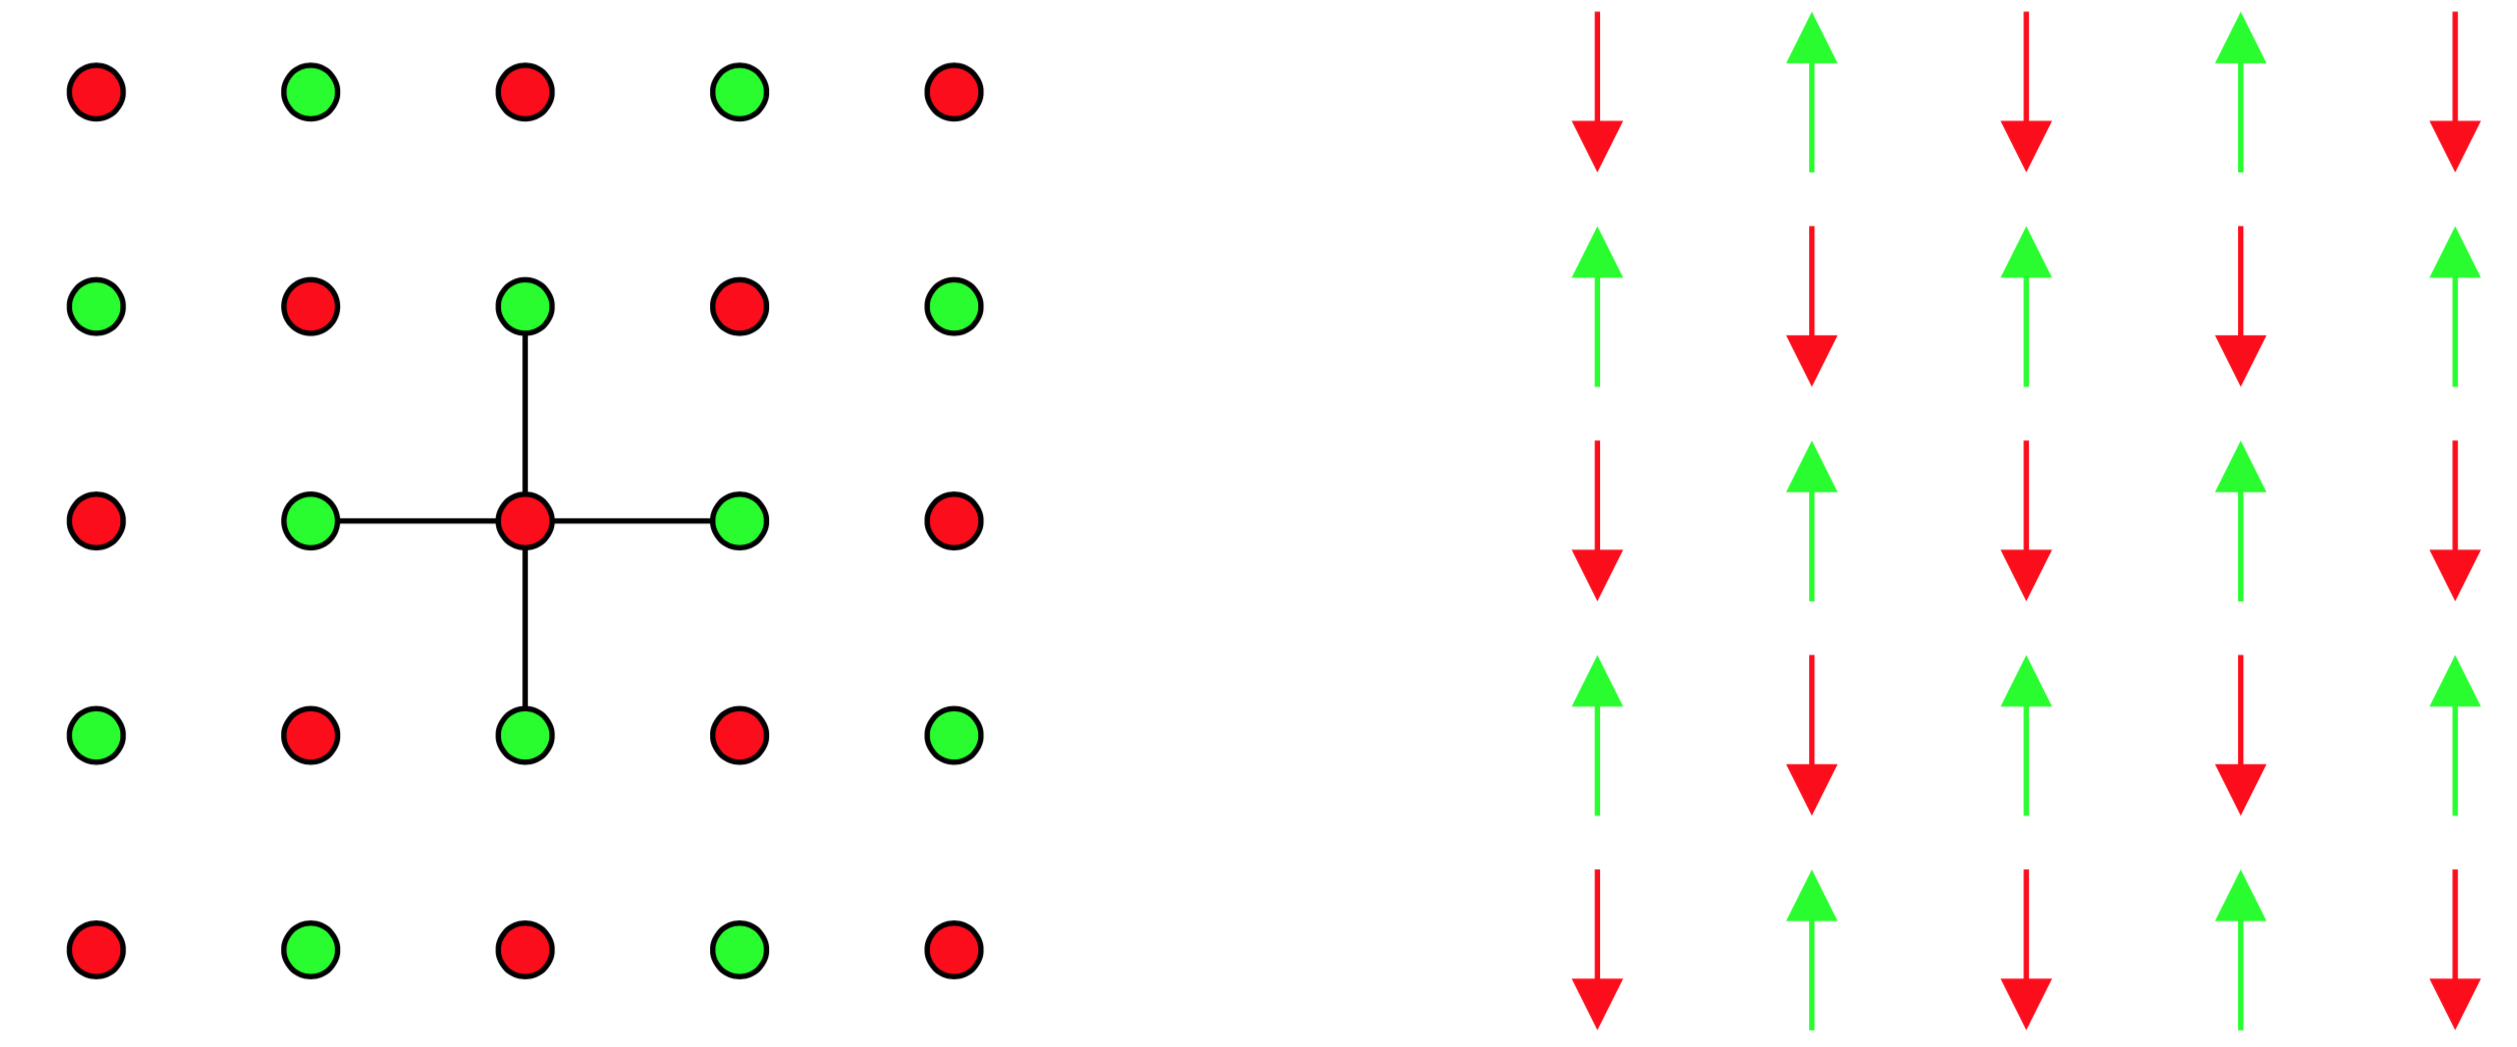
\includegraphics[width = 8cm]{Hubbard/bipartite}
\caption[Bipartite lattices and antiferromagnetic order.]{On the left, we see that the square lattice is bipartite.
The neighbors of a particular in the red sublattice all belong to the green sublattice.
The picture on the right,is meant to give some intuition on why the bipartite lattice favors AF order.
We represent a configuration where fermions of a given spin have as their neighbors only fermions of opposite spin (taken from \cite{alavi_quantum_2016}). }
\end{figure}

Introducing a particle-hole transformation (PHT)

\begin{equation}\label{eq:PHT}
d_{ i, \sigma}^\dagger = (-1)^i c_{i, \sigma} ,
\end{equation}
we exchange the role of annihilation and creation operators.

In fact, particles become holes and vice-versa: $d_{ i, \sigma}^\dagger d_{ i, \sigma} = 1 - c_{ i, \sigma}^\dagger c_{ i, \sigma} $, and the occupations $n = 0, 1$ are interchanged.

Consider a bipartite lattice.
Since in that case the factor $(-1)^i$ takes on $-1$ on one sublattice and $1$ on the other, the kinetic part of the Hamiltonian is invariant under a PHT:

\begin{equation}
c_{i, \sigma}^\dagger c_{j, \sigma} + c_{j, \sigma}^\dagger c_{i, \sigma} \mapsto (-1)^{i+j} ( d_{i, \sigma} d_{j, \sigma}^\dagger + d_{j, \sigma} d_{i, \sigma}^\dagger ) = d_{j, \sigma}^\dagger d_{i, \sigma} + d_{i, \sigma}^\dagger d_{j, \sigma}
\end{equation}

The PHS of the kinetic term can be incorporated into the interaction term by a shift in the chemical potential and by adding a constant to the Hamiltonian.
First, note that the term

\begin{equation*}
U ( n_{i,\uparrow} - \frac{1}{2} ) ( n_{i,\downarrow} - \frac{1}{2} )
\end{equation*}
is unchanged under a PHT.

Expanding this term, we obtain $U n_{i,\uparrow} n_{i,\downarrow} - \frac{U}{2} (n_{i,\uparrow} + n_{i,\downarrow}) + \frac{U}{4}$, which indeed differs by the original interaction term by a shift in the chemical potential plus a constant.
Thus,  particle-hole symmetric form of the Hamiltonian 

\begin{equation}
\mathcal{H} = -t \sum_{\left\langle i, j \right \rangle, \sigma} ( c_{i,\sigma} c_{j,\sigma}^\dagger + c_{j,\sigma}^\dagger c_{i,\sigma} ) + U \sum_{i} ( n_{i,\uparrow} - \frac{1}{2} ) ( n_{i,\downarrow} - \frac{1}{2} ) -\mu \sum_i ( n_{i,\uparrow} + n_{i,\downarrow} )
\end{equation}
is completely equivalent to the original Hamiltonian.

Under a PHT, the density transforms as $\rho \mapsto 2 - \rho$.
The Hamiltonian changes only in the chemical potential term: $\mu \mapsto -\mu$.
Thus, we have that $\rho (\mu) = 2 - \rho (-\mu)$, and at $\mu = 0$, we have half filling: $\rho = 1$.
This reasoning is valid for any $\beta$, $t$, or $U$, which implies that the phase diagram of the Hubbard model must be symmetric about half filling.
Suppose you added next nearest neighbor (NNN) hoppings $t'$ \footnote{On the square lattice, this corresponds to connecting sites across the diagonal of each square.}.
Then, PHS would be broken, and the phase diagram would no longer be symmetric about $\mu = 0$.
Indeed, a modified version of the Hubbard model with NNN hoppings is often used to model cuprate superconductors, and this lack of symmetry is consistent with the fact that hole- and electron-doped cuprates have different properties. 
\section{Mott insulators}\label{sec:mott}

Band theory was found to be flawed soon after it was introduced.
The picture it proposes is simple and generally works pretty well.
It is based on considering the electrons to be independently moving under the constant background potential created by the ions.
The solutions of the Schr\"odinger for free electrons in a periodic potential $U(\bm r)$, such that $U(\bm r) = U(\bm r + \bm R)$,

\begin{equation}\label{eq:schrodinger}
\bigg[ -\frac{1}{2m} \nabla^2 + U(\bm r) \bigg] \psi (\bm r) = \varepsilon \psi (\bm r)
\end{equation}
are given by Bloch's theorem: $\psi_{\bm k} (\bm r) = e^{i\bm k \cdot \bm r} u_{\bm k} (\bm r)$.
Note that we made $\hbar = 1$.
Replacing this wave function in equation (\ref{eq:schrodinger}), we obtain a differential equation for $u_{\bm k} (\bm r)$, which has in general an infinite number of solutions.
We label them with an index $n$, which we call the band index.
To each solution there corresponds a function $\varepsilon_{n\bm k}$.
The set of these functions is known as the band structure.
Since electrons are taken to be independent in band theory, the N-electron eigenstates are obtained by placing an electron in each quantum state.
Each state is labelled by its energy $\varepsilon_{n\bm k \sigma}$.
Since our model Hamiltonian does not couple spins (via an electron interaction, for example) and assuming there is no external magnetic field and that the system has an inversion center, we have $\varepsilon_{n\bm k \uparrow} = \varepsilon_{n\bm k \downarrow}$.
In general there might be energies for which there is no corresponding $\varepsilon_{n\bm k \sigma}$.
These form intervals called forbidden bands\footnote{We disregard surface states that may have energies that fall in the forbidden bands.}.
Thus, the ground state of our model may be obtained by filling the energy levels starting from the lowest energy state.
Two cases are particularly relevant:
\begin{itemize}
\item Every band is either fully occupied or empty.
The first excited state differs from the ground state by $\Delta$, the separation between the last fully occupied band and the first empty band.
It is then impossible to induce the motion of the electrons by applying an arbitrarily small voltage.
This is what it means to be an \emph{insulator}.
Since there $2N$ states per band, this is not possible unless the number of electrons per unit cell is an even integer.
\item One or more of the bands are partially filled.
The energy of occupied state of higher energy is named the Fermi energy $\varepsilon_F$.
In this case, the separation between the ground state and the first excited state tends to $0$ in the thermodynamic limit, $N \rightarrow \infty$.
The system may then respond to infinitesimal excitations, which is the definition of a metal.
\end{itemize}

Band theory made it possible to predict whether a solid would be a metal or an insulator.
However, its success rests crucially on the independent electron approximation.
Thus, it is not surprising that for compounds with strongly correlated electrons the theory might fail \cite{mila_physique_2007}.
The Coulomb interaction is in general non negligible, and the effects it leads to are not captured by a mean field approach.
One must resort to many-body theory.
An example of a many-body effect that band theory doesn't capture is (conventional) superconductivity.
However, this does not deem band theory useless.
In fact, the superconducting phase arises due to an instability of a state that is itself well described by band theory \cite{gennes_superconductivity_1999}.
A far greater failure of band theory is that predicts certain compounds with an odd number of electrons per unit cell, such as \chem{NiO} and \chem{La_2 Cu O_4},  to be metals, while in fact  they turn out to be (Mott) insulators.
Mott devised a simple argument to justify this failure.
It is based on considering the elementary electronic excitations of a solid composed by hydrogen atoms as a function of the distance between atoms.

Consider a hypothetical solid consisting of a square lattice with hydrogen atoms on its points.
Each unit cell has one hydrogen atom, and consequently one electron.
Band theory would predict such a solid to be a metal.
However, if the lattice parameter $a$ is large enough, the solid cannot remain a metal.
There must be some value of the lattice parameter $a = a_c$ for which the system becomes an insulator.
When current flows through a sample of this solid, electrons hop consecutively, reaching positions that can be quite far on the lattice.
For a metal, this process occurs even when exciting the system with an infinitesimal amount of energy.
How much energy do we need to provide for this process to occur?

\begin{figure}[ht!]\label{hubbardOneHoleOneDoublyOc}
\centering
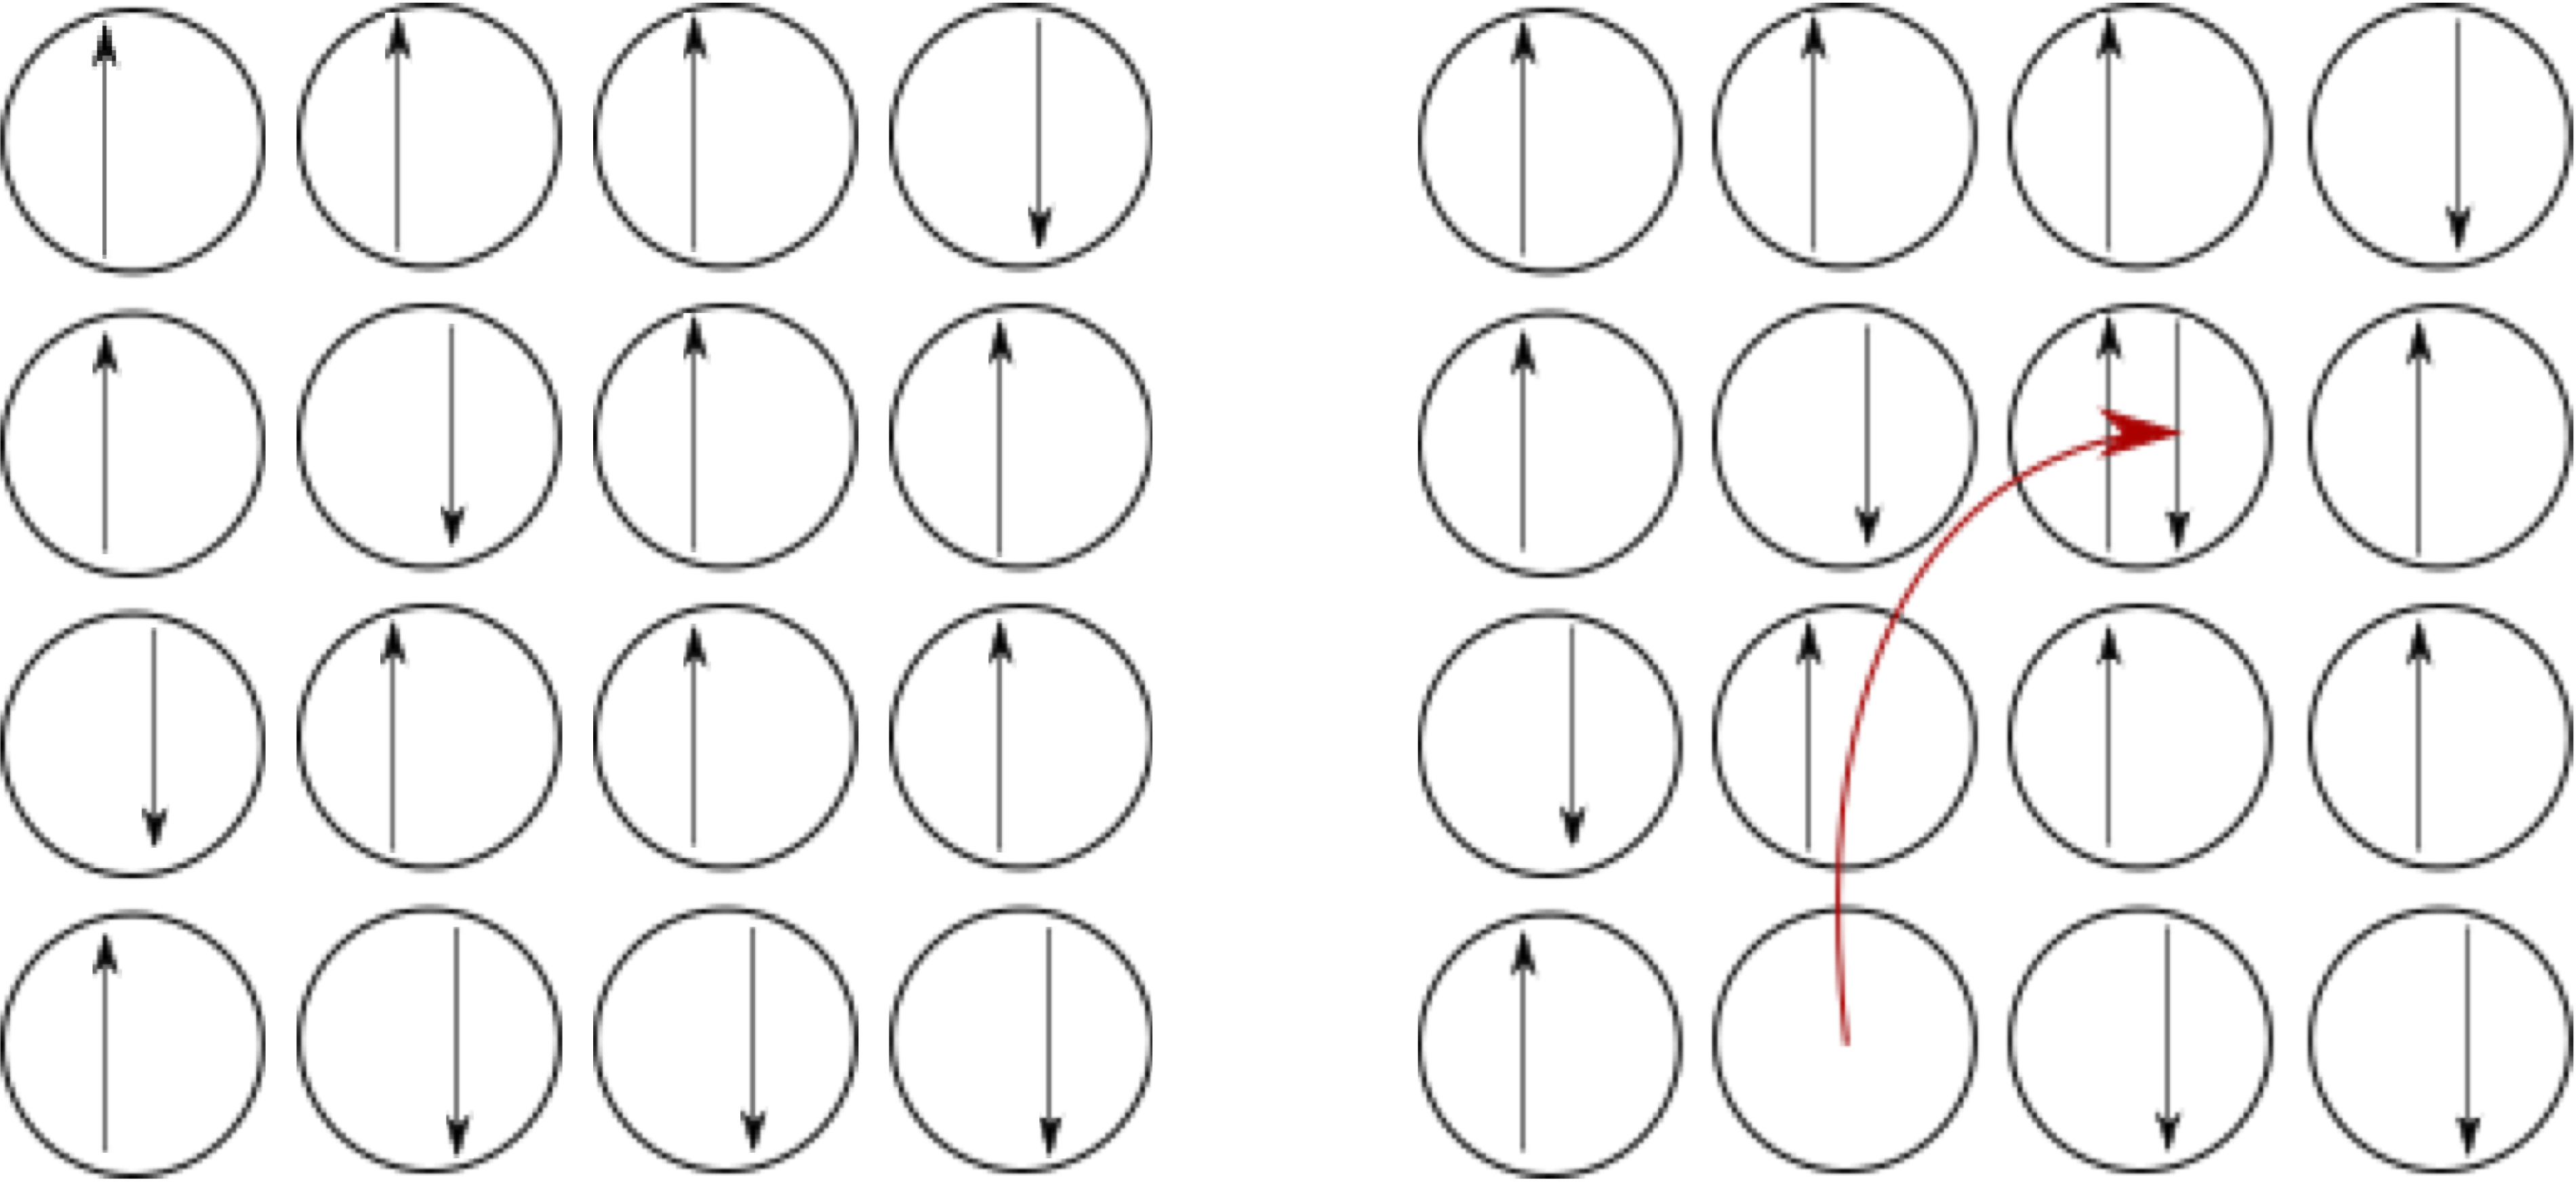
\includegraphics[width = 9cm]{Hubbard/hubbardOneHoleOneDoublyOcV2.png}
\caption[Configuration of the Hubbard model on the square lattice with a hole and a doubly occupied site.]{On the right, a configuration on the square lattice with a hole and a doubly occupied site obtained by delocalization of the spin down electron on the left.}
\end{figure}

If $a$ is large, we have essentially one electron per site at the start.
When an electron is displaced, we end up with a hole and a doubly occupied site.
The potential energy of such a state is

\begin{equation}
E_{H^-} + E_{H^+} - 2 E_H 
\end{equation}

Due to the Coulomb repulsion between the two electrons in $H^-$, this quantity is strictly positive.
Call it $U > 0$.
On the other hand, the system also has kinetic energy: both the hole and the doubly occupied site can delocalize.
Let $W$ be the bandwidth corresponding to the delocalization of an electron on the lattice.
Both the hole and the doubly occupied will stay at the bottom of the band and gain an energy $W/2$ (assuming that this delocalization is of the same order of magnitude).
The dominant transfer integral $-t$ is between nearest neighbors.
The dispersion relation then reads

\begin{equation}
\varepsilon_{\bm k} = -2 t ( \cos k_x + \cos k_y ) 
\end{equation}

The bandwidth is then $W = 8 t$.
The energy of a configuration with a hole and a doubly occupied site is

\begin{equation}
\Delta_c = U - W ,
\end{equation}
where $U$ is practically independent of the lattice parameter $a$.
The bandwidth $W$, however, depends strongly on $a$.
When $a \gg a_0$, where $a_0$ is the Bohr radius, the transfer integral is exponentially small, because only the exponential tails of the wave functions are relevant.
In this limit, $\Delta_c \approx U$ is a large, positive number, and the system is an insulator.
This type of insulator is called a Mott insulator, and $\Delta_c$ is called the charge gap.
As $a$ decreases, $t$ increases, and there must be a critical value $a_c \sim a_0$, for which $U = W$.
Below this value, the computation of $\Delta_c$ is not valid anymore because the gap cannot be negative.
Thus, there must be a metal-insulator transition.
It is possible to see this transition if we apply enough pressure to a Mott insulator so as to decrease $a$ and increase $t$.
A transition of this type was first seen in the 1970's for $V_2 O_3$\footnote{Of course, the transition is not so easy to describe.
However, this simple argument provides an intuitive picture.}.
There is a fundamental difference between a band insulator and a Mott insulator.
While we must pay an energy $\Delta_c$ to make a charge excitation, this is not the cost of a spin excitation: we can flip the spin of an electron without creating a doubly occupied site.
The fluctuations of both charge and spin due to the electron interactions may then lead to magnetic behavior characteristic of this type of systems.
\section{Exact solutions for simple cases}\label{sec:exactSolutions}

In PHS form, the Hubbard Hamiltonian may then be written as a sum of kinetic, chemical and potential energy terms, respectively:

\begin{equation}\label{eq:hubbard}
\mathcal{H} = \mathcal{H}_K + \mathcal{H}_\mu + \mathcal{H}_V ,
\end{equation}
defined as

\begin{equation}\label{eq:def_energies}
\begin{split}
\mathcal{H}_K &= -t \sum_{\left\langle i, j \right \rangle, \sigma} ( c_{i,\sigma} c_{j,\sigma}^\dagger + c_{j,\sigma}^\dagger c_{i,\sigma} ) \\
\mathcal{H}_\mu &= -\mu \sum_i ( n_{i,\uparrow} + n_{i,\downarrow} ) \\
\mathcal{H}_V &= U \sum_{i} ( n_{i,\uparrow} - \frac{1}{2} ) ( n_{i,\downarrow} - \frac{1}{2} )
\end{split} ,
\end{equation}
where:

\begin{itemize}
\item $i$ and $j$ label sites on the lattice.
\item $c_{i,\sigma}^{(\dagger)}$ is an operator that annihilates (creates) an electron with spin $\sigma$ on site $i$.
\item $n_{i,\sigma}$ is the number operator counting the number of electrons of spin $\sigma$ on site $i$ (either 0 or 1).
\item $t$ is the hopping parameter related to the kinetic energy of the electrons. It is determined by the overlap of the atomic wave functions on neighboring sites $\left\langle i, j \right\rangle$.
\item $U$ is the repulsive Coulomb interaction between electrons on the same lattice site. Whenever a site $i$ has two electrons, there is a local repulsion between them corresponding to an energy cost $U n_{i \uparrow} n_{i \downarrow}$. The constant $1/2$ terms serve to recast the Hamiltonian in particle-hole symmetric form.
\item $\mu$ is the chemical potential controlling the electron number (or density).
\end{itemize}

A given physical observable of interest $\mathcal{O}$, such as the spin-spin correlation, or the magnetic susceptibility may be computed formally by

\begin{equation}
\left\langle \mathcal{O} \right\rangle = \text{Tr} ( \mathcal{O} \mathcal{P} )
\end{equation}
where

\begin{equation}\label{eq:projection}
\mathcal{P} \equiv \frac{1}{Z} e^{-\beta \mathcal{H} } , \text{ with } Z = \text{Tr} ( e^{-\beta \mathcal{H} } )
\end{equation}

The trace is taken over the Hilbert space corresponding to all possible configurations of the lattice occupation. Defining an orthonormal basis of this Hilbert space $\{ | \psi_\alpha \rangle | \alpha = 1, ... D \} $, where $D$ is the dimension of the Hilbert space, the partition function reads

\begin{equation}\label{eq:z_asEigen}
\Tr ( e^{-\beta \mathcal{H} } )= \sum_\alpha \left\langle \psi_\alpha | e^{-\beta \mathcal{H} } | \psi_\alpha \right\rangle
\end{equation}

There are four possible states at each site in the Hubbard model: $\left| \,\, \right\rangle$, $\left|\uparrow \right\rangle$, $\left|\downarrow\right \rangle$, $\left|\uparrow \downarrow \right\rangle $, corresponding, respectively, to no electron, a spin up or spin down electron, and two electrons of opposite spin occupying the site. The potential energy operator acts as follows

\begin{equation}
U (n_{i\uparrow} - \frac{1}{2} ) ( n_{i\downarrow} - \frac{1}{2} ) 
\begin{cases}
\left| \,\, \right\rangle = \frac{U}{4} \left| \,\, \right\rangle \\
\left|\uparrow \right\rangle = -\frac{U}{4} \left|\uparrow \right\rangle \\
\left|\downarrow\right \rangle = -\frac{U}{4} \left|\downarrow\right \rangle \\
\left|\uparrow \downarrow \right\rangle = \frac{U}{4} \left|\uparrow \downarrow \right\rangle \\
\end{cases}
\end{equation}

Singly occupied states ($\left|\uparrow \right\rangle$, $\left|\downarrow\right \rangle$) have lower energy and are thus more likely to occur. They correspond to nonzero magnetization $m = n_{\uparrow} - n_{\downarrow}$, which is favored by the Hubbard interaction $U$. A relevant question is whether or not the spins order in space when $t \neq 0$ and to what extent.

Let us now establish our notations for second quantized operators to introduce a different representation of electronic states on the lattice. The fermionic annihilation and creation operators anticommute.

\begin{equation}
\{ c_{j\sigma} , c_{l \sigma'}^\dagger \} = \delta_{jl} \delta_{\sigma\sigma'}
\end{equation}

The $c$-operator algebra is further defined by the vanishing of all other anticommutators.

\begin{equation}\label{eq:fermion_anticom}
\{ c_{j\sigma}^{(\dagger)} , c_{l \sigma'}^{(\dagger)} \} = 0
\end{equation}

Note that taking $l = j$ and $\sigma = \sigma'$ in equation (\ref{eq:fermion_anticom}) for the $c^\dagger$-operators, we recover Pauli's exclusion principle since $(c_{j\sigma}^\dagger)^2 = 0$. If we omit the site $i$ and spin $\sigma$ indices, a convenient way of specifying states on the lattice is

\begin{equation}
\begin{split}
&\left| 0 \right\rangle : \text{unoccupied state - no electron} \\
&\left| 1 \right\rangle : \text{occupied state - one electron}
\end{split}
\end{equation}
so that a generic state may be written as a product of the states above $\otimes_{i=1}^{N} \otimes_{\sigma = \pm 1/2} \left| n \right\rangle_{i, \sigma}$ at each site for each spin state, where $n= 0, 1$. For example, one such state is

\begin{equation}
\left| 0 \right\rangle_{1, 1/2} \left| 1 \right\rangle_{1, -1/2} \left| 0 \right\rangle_{2, 1/2} \left| 0 \right\rangle_{2, -1/2} ... \left| 0 \right\rangle_{N, 1/2} \left| 1 \right\rangle_{N, -1/2}  ,
\end{equation}
where $N$ is the number of sites on the lattice.

The creation and annihilation operators act as follows

\begin{equation}
c \left| 0 \right\rangle = 0 \quad c^\dagger \left| 0 \right\rangle = \left| 1 \right\rangle \quad c \left| 1 \right\rangle = \left| 0 \right\rangle \quad c^\dagger \left| 1 \right\rangle = 0
\end{equation}

Thus, the eigenstates of the number operator are $\left| 0 \right\rangle, \left| 1 \right\rangle$:

\begin{equation}
n \left| 0 \right\rangle = 0 \quad n \left| 1 \right\rangle = \left| 1 \right\rangle
\end{equation}

Moreover, the operator $c_i^\dagger c_{i+1}^\dagger$, corresponding to the hopping from site $i+1$ to $i$, i.e. to the kinetic energy of the electrons on neighboring sites, acts as follows (ignoring spin):

\begin{equation}
c_i^\dagger c_{i+1}^\dagger \begin{cases}
\left|0 0 \right\rangle = 0 \\
\left|1 0 \right\rangle =  0 \\
\left|0 1 \right\rangle =  \left| 1 0 \right\rangle \\
\left|1 1 \right\rangle =  c_i^\dagger \left| 1 0  \right\rangle = 0 \\
\end{cases}
\end{equation}

The operator annihilates the particle at $i+1$ and creates it back at $i$, i.e. the electron hops from $i+1$ to $i$.

\subsection{The purely atomic $\frac{t}{U} = 0$ limit}

When $t = 0$, the site index may be omitted since the Hamiltonian is a sum of operators solely at site $i$. Hence, we have $[ \mathcal{H}, n_{i,\sigma} ] = 0 \forall i $, and the eigenstates of $\mathcal{H}$ are also eigenstates of all number operators at the different sites in the lattice. Thus, in the single site limit, we obtain

\begin{equation}
\mathcal{H} = U (n_\uparrow - \frac{1}{2} ) (n_\downarrow - \frac{1}{2} ) - \mu ( n_\uparrow + n_\downarrow )
\end{equation}
which acts as follows (using the eigenstates of $n_\sigma$)

\begin{equation}
\mathcal{H} \begin{cases}
\left| \,\, \right\rangle = \frac{U}{4} \\
\left| \uparrow \right\rangle = \bigg( \frac{U}{4} - (\mu + \frac{U}{2} ) \bigg) \left| \uparrow \right\rangle \\
\left| \downarrow \right\rangle = \bigg( \frac{U}{4} - (\mu + \frac{U}{2} ) \bigg) \left| \downarrow \right\rangle \\
\left| \uparrow \downarrow \right\rangle = \bigg( \frac{U}{4} - 2 \mu \bigg) \left| \uparrow \downarrow \right\rangle
\end{cases}
\end{equation}

Thus, the Hamiltonian is diagonal in the basis $\{\left| \psi_\alpha \right\rangle \} = \left| \,\, \right\rangle, \left|\uparrow \right\rangle, \left|\downarrow\right \rangle, \left|\uparrow \downarrow \right\rangle $:

\begin{equation}
\begin{split}
&\bigg[ \mathcal{H}_{\rho\gamma} \bigg] = \bigg[ \left\langle \psi_\rho \left| \mathcal{H} \right| \psi_\gamma \right\rangle \bigg] \\
&= \text{diag}\bigg(\frac{U}{4}, \frac{U}{4} - (\mu + \frac{U}{2} ), \frac{U}{4} - (\mu + \frac{U}{2} ), \frac{U}{4} - 2 \mu \bigg) ,
\end{split}
\end{equation}
which means that $e^{-\beta \mathcal{H} }$ is also diagonal:

\begin{equation}
e^{-\beta \mathcal{H} } = e^{-\beta U / 4}  \text{diag}\bigg(1,  e^{\beta(\mu + \frac{U}{2})}, e^{\beta(\mu + \frac{U}{2})},  e^{2\beta \mu} \bigg)
\end{equation}
and this is one of the rare situations in which it is possible to explicitly write down a closed form for the partition function.

\begin{equation}
\begin{split}
Z &= \text{Tr} ( e^{-\beta\mathcal{H} } ) = \sum_\alpha \left\langle \psi_\alpha \left|e^{-\beta \mathcal{H} } \right| \psi_\alpha \right\rangle \\
&= e^{-\beta U / 4} \bigg(1 + 2 e^{\beta(\mu + \frac{U}{2})} + e^{2 \beta \mu} \bigg)
\end{split}
\end{equation}

Moreover, some of the observables that were mentioned before are explicitly computable. This is because due to the diagonal form of $\mathcal{H}$, the expressions defining these observables greatly simplify.

\begin{equation}
\begin{split}
\mathcal{H} e^{-\beta\mathcal{H} } &\mapsto e^{-\beta U / 4}  \text{diag}\bigg(\frac{U}{4}, (-\mu - \frac{U}{4})  e^{\beta(\mu + \frac{U}{2})} (-\mu - \frac{U}{4}) e^{\beta(\mu + \frac{U}{2})}, (\frac{U}{4} - 2\mu ) e^{2\beta \mu} \bigg) \\
n_{\uparrow} e^{-\beta\mathcal{H} } &\mapsto e^{-\beta U / 4}  \text{diag}\bigg(0, e^{\beta(\mu + \frac{U}{2})}, 0,  e^{2\beta \mu} \bigg) \\
n_{\downarrow} e^{-\beta\mathcal{H} } &\mapsto e^{-\beta U / 4}  \text{diag}\bigg(0, 0, e^{\beta(\mu + \frac{U}{2})},   e^{2\beta \mu} \bigg) \\
n_{\uparrow} n_{\downarrow} e^{-\beta\mathcal{H} } &\mapsto e^{-\beta U / 4}  \text{diag}\bigg(0, 0, 0,   e^{2\beta \mu} \bigg) \\
\end{split}
\end{equation}

From these we can compute some traces which we shall find useful to obtain averages of various observables.

\begin{equation}
\begin{split}
&\Tr \bigg( \mathcal{H} e^{-\beta\mathcal{H} } \bigg) = e^{-\beta U / 4} \bigg(\frac{U}{4} + 2 (-\mu - \frac{U}{4})  e^{\beta(\mu + \frac{U}{2})} + (\frac{U}{4} - 2\mu ) e^{2\beta \mu} \bigg) \\
&\Tr \bigg( (n_\uparrow + n_\downarrow ) e^{-\beta\mathcal{H} } \bigg) = e^{-\beta U / 4} \bigg(2 (-\mu - \frac{U}{4})  e^{\beta(\mu + \frac{U}{2})} + (\frac{U}{4} - 2\mu ) e^{2\beta \mu} \bigg) \\
&\Tr \bigg( n_\uparrow n_\downarrow \bigg) = e^{-\beta U/4} e^{2\beta\mu}
\end{split}
\end{equation}

The bottom line is that we are able to obtain \emph{exact} expressions for

\begin{enumerate}
\item the one-site density $\rho = \left\langle n_\uparrow \right\rangle + \left\langle n_\downarrow \right\rangle$, measuring the average occupation of each site.
\begin{equation}
\begin{split}
\rho &= \frac{\text{Tr} \big[ (n_\uparrow + n_\downarrow ) e^{-\beta\mathcal{H}} \big]}{Z} \\
&= \frac{2 e^{\beta(\frac{U}{2} + \mu)} + 2 e^{2\beta\mu}}{1 + 2 e^{\beta(\mu + \frac{U}{2})} + e^{2 \beta \mu}}
\end{split}
\end{equation}

Note that when there is no chemical potential $\mu = 0$, we have $\rho = 1$ for any $U$, or $\beta$. This corresponds to half filling: the density of electrons is half its maximum possible value.

\begin{figure}[H]
	\centering
\hspace{12mm}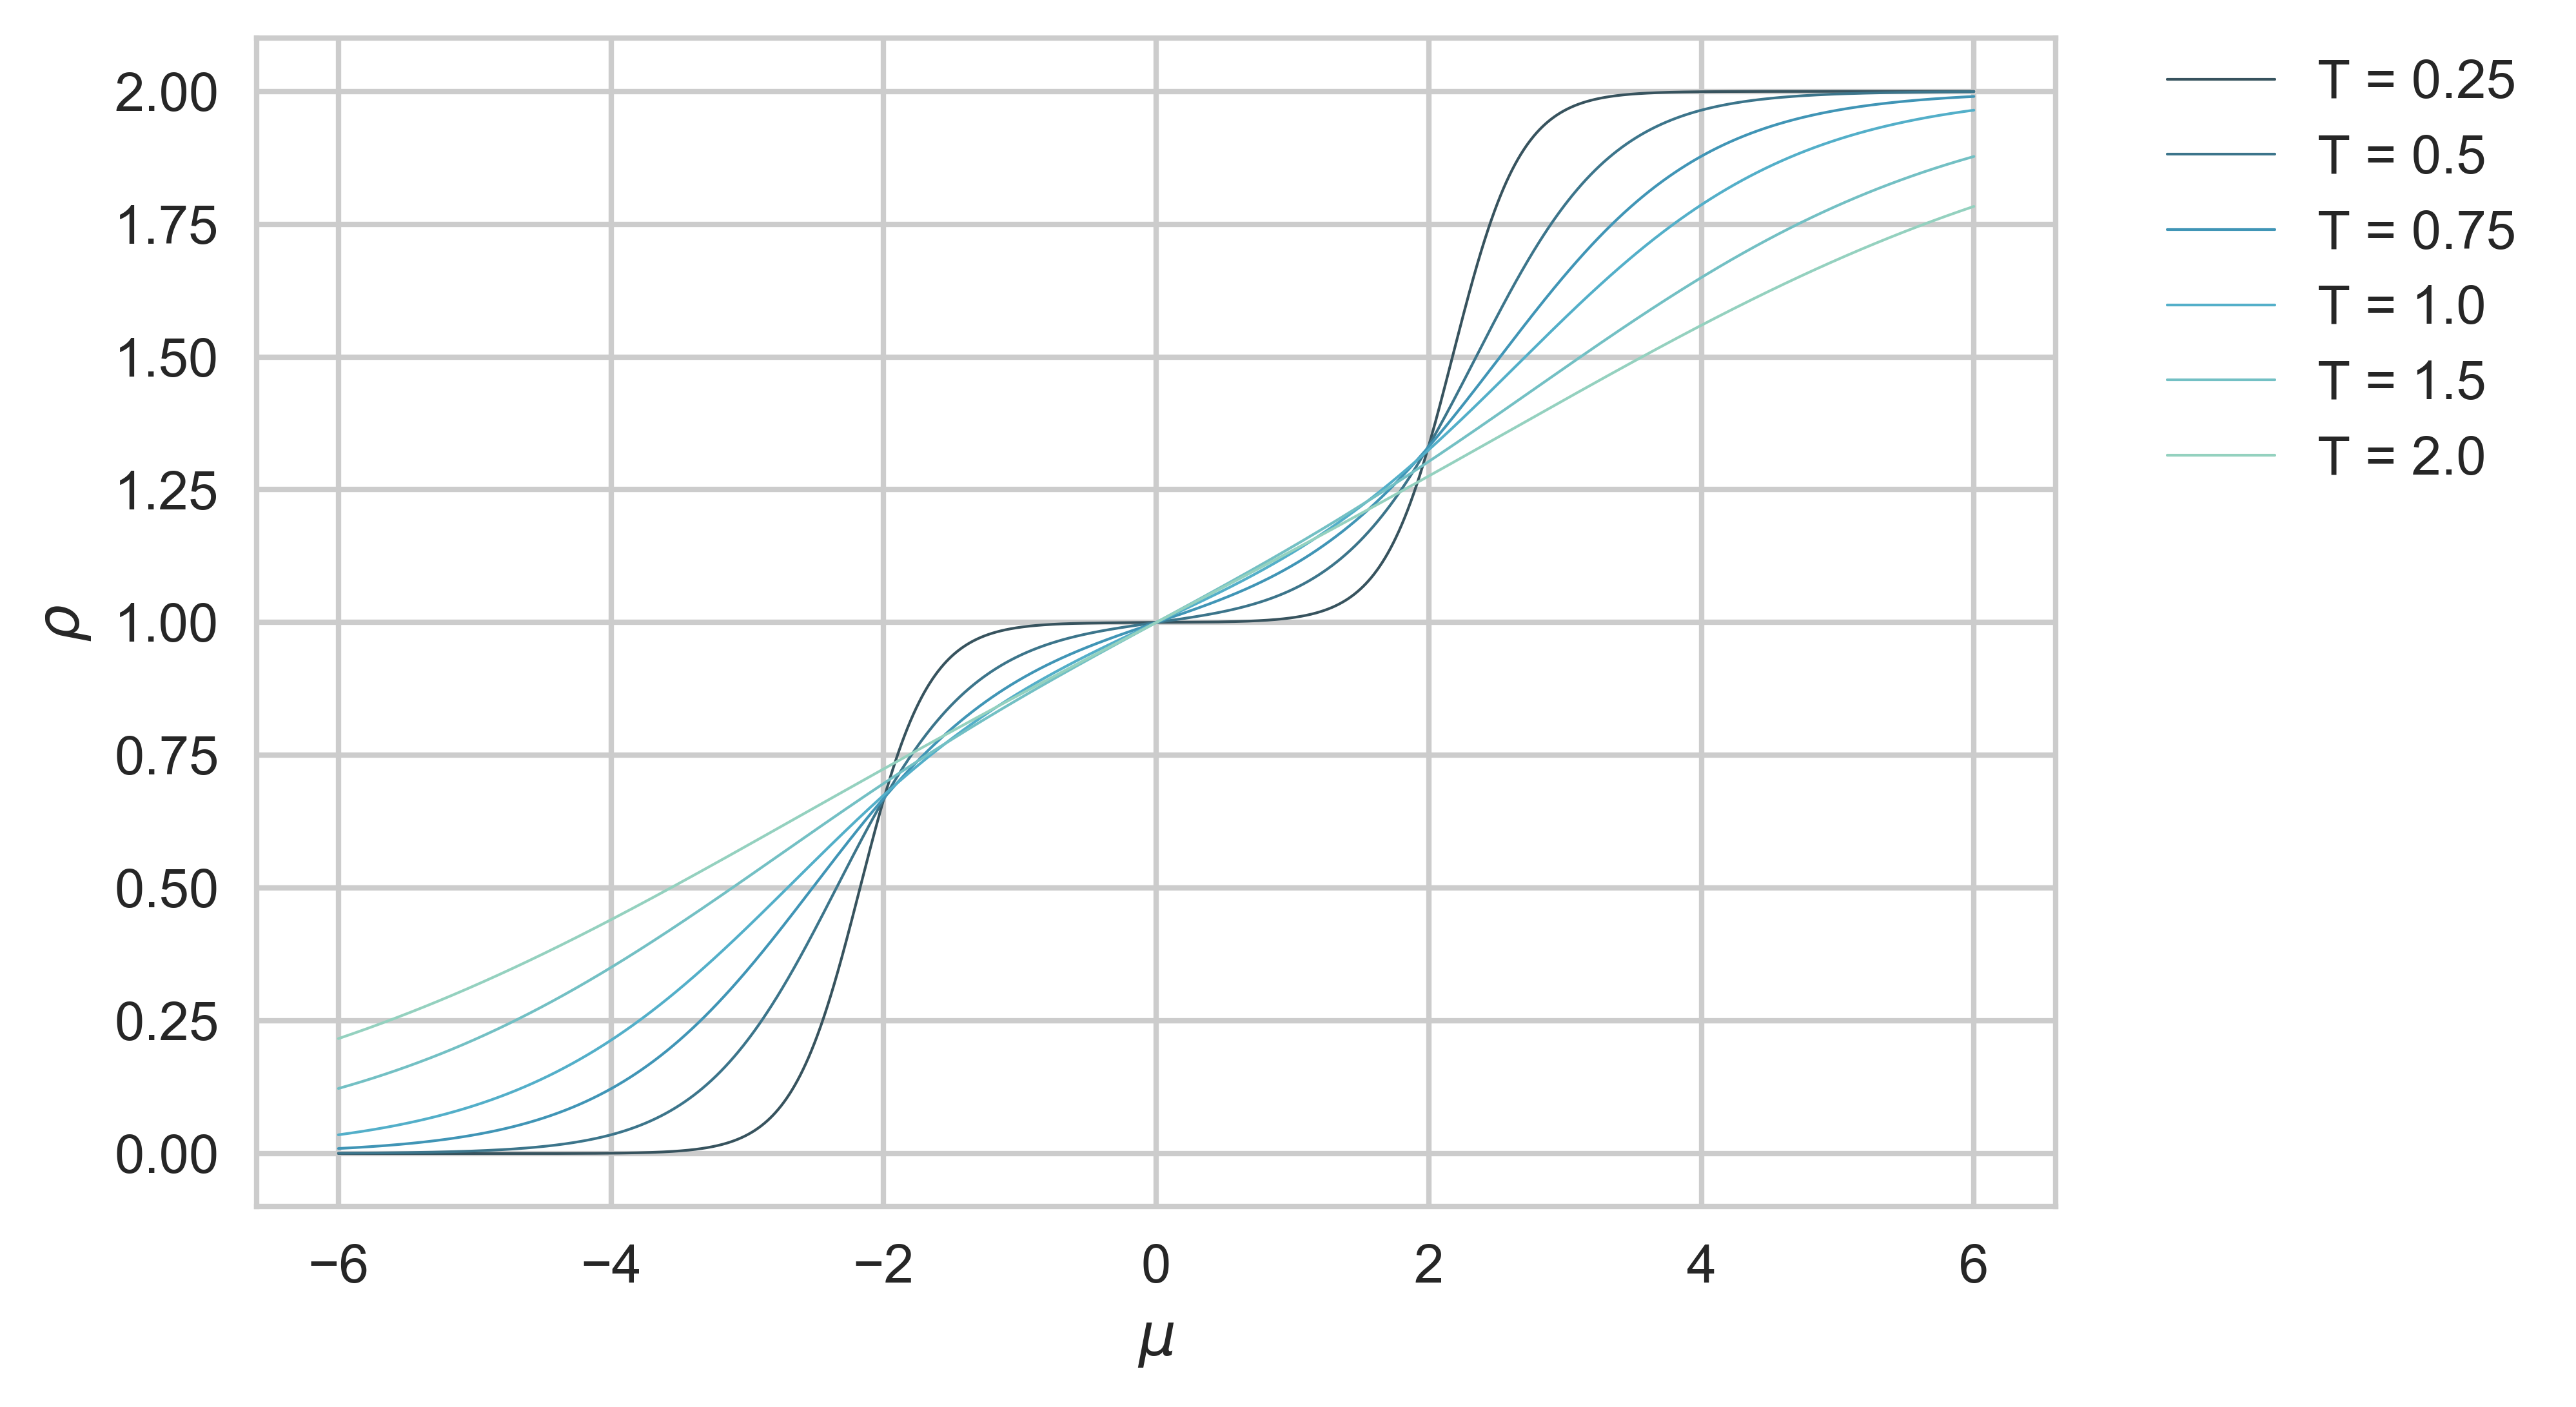
\includegraphics[width=0.83\linewidth]{Figures/HubbardModel/rhoVsMu.png}
	\caption[]{}
	\label{fig:rhoVsMu}
\end{figure}

\item the one-site energy $E = \left\langle \mathcal{H} \right\rangle$.
\begin{equation}
\begin{split}
E &= \frac{\text{Tr}\bigg( \mathcal{H}e^{-\beta\mathcal{H} } \bigg)}{Z} \\
&= \frac{ \frac{U}{4} + 2 ( -\mu - \frac{U}{4} ) e^{\beta(\frac{U}{2} + \mu )} + (\frac{U}{4} - 2\mu ) e^{2\beta\mu}}{1 + 2 e^{\beta (\frac{U}{2} + \mu )} + e^{2\beta\mu} } \\
&= \frac{ \frac{U}{4} ( 1 + 2 e^{\beta (\frac{U}{2} + \mu )} + e^{2\beta\mu} )}{1 + 2 e^{\beta (\frac{U}{2} + \mu )} + e^{2\beta\mu} } + \frac{2(-\mu - \frac{U}{4}) e^{\beta(\frac{U}{2} + \mu)} - 2\mu e^{2\beta\mu} - 2\frac{U}{4} e^{\beta (\frac{U}{2} + \mu)} }{1 + 2 e^{\beta (\frac{U}{2} + \mu )} + e^{2\beta\mu}} \\
&= \frac{U}{4} - \frac{ (2\mu - U) e^{\beta(\frac{U}{2} + \mu) } + 2\mu e^{2\beta\mu} }{1 + 2 e^{\beta (\frac{U}{2} + \mu )} + e^{2\beta\mu} }
\end{split}
\end{equation}
which at half filling becomes

\begin{equation}
E = \frac{U}{4} - \frac{U}{2 ( 1 + e^{-\beta U /2} )}
\end{equation}

\item the double occupancy $\left\langle n_\uparrow n_\downarrow \right\rangle$.

\begin{equation}
\left\langle n_\uparrow n_\downarrow \right\rangle = \frac{\text{Tr} \big[ n_\uparrow n_\downarrow \big]}{Z} = \frac{e^{2\beta\mu}}{1 + 2 e^{\beta (\frac{U}{2} + \mu )} + e^{2\beta\mu}}
\end{equation}
which, at half filling, simplifies to

\begin{equation}
\left\langle n_\uparrow n_\downarrow \right\rangle = \frac{1}{2 ( 1 + e^{\beta U/2} )}
\end{equation}

Note that as either $U$ or $\beta$ increase the double occupancy tends to zero.
\end{enumerate}

\subsection{The non-interacting $\frac{t}{U} \rightarrow \infty$ limit}

In the $\frac{t}{U} \rightarrow \infty$ limit, the spin spaces become independent, and they may be considered separately. Thus, we omit the spin indices of the operators in the Hamiltonian:

\begin{equation}
\mathcal{H} = -t \sum_{\left\langle i, j \right\rangle} \big( c_i^\dagger c_j + c_j^\dagger c_i \big) - \mu \sum_i n_i
\end{equation}
which may be recast as a bilinear form

\begin{equation}
\mathcal{H} = \bm c^\dagger ( -t \bm K - \mu \bm I ) \bm c ,
\end{equation}
where

\begin{equation}
\bm c = \bigg[ c_1 \,\, c_2 \,\, ... \,\, c_N \bigg]^T \quad \bm c^\dagger = \bigg[c_1^\dagger \,\, c_2^\dagger \,\, ... c_N^\dagger \bigg]
\end{equation}
and $\bm I$ is the identity matrix. We also defined a matrix of zeros and ones specifying the hopping geometry, $\bm K$. When writing down $\bm K$, we must specify the boundary conditions. Periodic boundary conditions (PBCs) preserve a system's translational invariance and are advantageous because they reduce finite size effects. An example of a quantity which is measured more accurately is energy. In the thermodynamic limit, $N \rightarrow \infty$, the measured energy differs from the actual value by a correction of order $\mathcal{O}(\frac{1}{N^2})$ with PBCs \textcolor{red}{missing citation}, while for open boundary conditions (OBCs), the correction is of order $\mathcal{O}(\frac{1}{N})$. Additionally, PBCs have the property of giving site independent observables. For example, the electron density per site does not vary with PBCs, but it varies with the distance to the edges of the lattice when we use OBCs.

Consider a rectangular two-dimensional lattice with $N_x \times N_y$ sites. Then, we have $\dim(\bm K) = N_x N_y \times N_x N_y $, and

\begin{equation}
\bm K = \bm I_y \otimes \bm K_x + \bm I_x \otimes \bm K_y ,
\end{equation}
where $\bm I_{x, y}$ are identity matrices of dimension $N_{x, y}$, respectively, and $\bm K_{x, y}$ are the hopping matrices in the $x$ and $y$-directions respectively.

For lattices in 1D or 2D, it is possible to find an exact eigendecomposition

\begin{equation}
\bm K = \bm F^T \bm \Lambda \bm F \quad \text{with}  \quad \bm F^T \bm F = \bm I ,
\end{equation}
where $\bm \Lambda = \text{diag}(\lambda_k)_{k = 1}^{N_x N_y}$ is a diagonal matrix of eigenvalues of $\bm K$. The Hamiltonian is diagonalized:

\begin{equation}\label{eq:quadraticH}
\mathcal{H} =\tilde{\bm c}^\dagger \big( -t \bm K - \mu \bm I \big) \tilde{\bm c} = \sum_k \varepsilon_k \tilde{n}_k ,
\end{equation}
where $\tilde{\bm c} = \bm F \bm c$ and $\tilde{\bm c}^\dagger = (\bm F \bm c)^\dagger$, and

\begin{equation}
\varepsilon_k = -t \lambda_k - \mu \quad \tilde{n}_k = \tilde{c}_k^\dagger \tilde{c}_k
\end{equation}

The $\tilde{c}$-operators are equally valid electron creation/annihilation operators, obeying the same anticommutation relations as the original operators $c_i$. While the original operators create/annihilate particles at specific (spatial) sites, the new ones create/annihilate particles with momentum $k$. Both sets of operators describe the same physics, however the interaction term in the Hubbard model is fairly complex to write in momentum space so it is not possible to apply this procedure to diagonalize it.

\bigskip

Now, it turns out that it is easy to evaluate the partition function for quadratic Hamiltonians. If $\mathcal{H} = \bm c^\dagger \bm H \bm c$, where $\bm H$ is a $N \times N$ Hermitian matrix, then we have that

\begin{equation}\label{eq:trace_quadratic}
\text{Tr} \big[ e^{-\beta \mathcal{H} } \big] = \prod_{i=1}^N ( 1 + e^{-\beta \lambda_{k_i} } ) ,
\end{equation}
where $\lambda_{k_i}$ are the eigenvalues of $\bm H$.

We present a proof of this result in appendix \ref{ap:Zquadratic}.

Thus, this result suggests that if we are able to devise some approximation to transform the quartic term of the interacting Hubbard model in a quadratic form, then we can solve it.

To complete the solution of the non-interacting case we apply the result of equation (\ref{eq:trace_quadratic}) to compute the partition corresponding to the quadratic Hamiltonian defined in equation (\ref{eq:quadraticH}):

\begin{equation}
Z = \prod_k ( 1 + e^{-\beta \varepsilon_k} )
\end{equation}

Now that we have found a closed form solution for $Z$, it is again possible to find closed form expressions for observables of interest as well, namely:

\begin{enumerate}
\item the density, or average occupation of each site, $\rho$.

\begin{equation}
\rho = \left\langle n \right\rangle = \left\langle \tilde{n} \right\rangle = \frac{1}{N} \sum_{k=1}^N \left\langle \tilde{n}_k \right\rangle  = \frac{1}{N} \sum_{k=1}^N  \frac{1}{1 + e^{\beta\varepsilon_k}}
\end{equation}

\item the energy $E = \left\langle \mathcal{H} \right\rangle$.

\begin{equation}
E = \frac{1}{N} \sum_k \frac{\varepsilon_k}{1 + e^{\beta\varepsilon_k}}
\end{equation}

\item the equal-time Green's function, which plays a key role in computing other quantities, such as correlation functions.

\begin{equation}
G_{lj} = \left\langle c_l c_j^\dagger \right\rangle = \frac{1}{N} \sum_k e^{ i k \cdot ( l - j ) } ( 1 - f_k ),
\end{equation}
where $f_k = \big(1 + e^{\beta(\varepsilon_k - \mu)} \big)^{-1}$ is the Fermi-Dirac distribution (of course, here we consider half filling: $\mu = 0$). Note that the Green function, like the Hamiltonian, is translationally invariant: $G_{lj} = G_{l-j}$. If we use PBCs, no site is singled out, they are all equivalent and this behavior of the Green's function should become apparent.
\end{enumerate}
\section{Effective Heisenberg Hamiltonian}\label{sec:effectiveHeisenberg}

Mott insulators allow low energy magnetic excitations (spin flips). The insulating phase corresponds to a configuration where each atom has an odd number of electrons, let's say one. This electron may have its spin up or down. In the purely atomic limit $\frac{t}{U} \rightarrow 0$, the atoms are infinitely far, and the excitation spectrum is very simple. The ground state is highly degenerate: every configuration with one electron per site is a ground state. As a matter of fact, the ground state is $2^N$-fold degenerate. The first excited state corresponds to configurations with a hole and a doubly occupied site. Let us set the energy of the ground state to zero in our conventions.  The energy of these configurations is then $U$, and there are $N(N-1)2^{N-2}$ of them. This process of generating higher energy excitations may be continued.

When the atoms are brought together, the first effect is the lifting of the degeneracy of the ground state, i.e. the splitting of the subspace of energy $E = 0$ in more subspaces. The effective hamiltonian describing the lifting of the degeneracy of the lowest energy band is obtained by applying degenerate perturbation theory \cite{Mila2007} to the kinetic term of the Hubbard Hamiltonian\footnote{An alternative method would be to use a canonical transformation technique.}

\begin{equation}
\mathcal{H}_0 = - t \sum_{\left\langle i, j \right\rangle, \sigma} ( c_{i\sigma}^\dagger c_{j\sigma} + c_{j\sigma}^\dagger c_{i\sigma} ) 
\end{equation}

\subsection{Two-site calculation}

The effect of the hopping term is best understood in a minimal two-site example. There are four one-particle quantum states, represented by the action of the operators $c_{1,\uparrow}^\dagger$, $c_{1,\downarrow}^\dagger$, $c_{2,\uparrow}^\dagger$, $c_{2,\downarrow}^\dagger$ on the vacuum state. There are six two-particle states in the Fock space $\left| n_{1\uparrow} \,  n_{1\downarrow} \,  n_{2\uparrow} \, n_{2\downarrow} \right\rangle$:

\begin{equation}
\begin{split}
\left| 1 \right\rangle &\equiv \left| 1, 0, 1, 0 \right\rangle = c_{1\uparrow}^\dagger c_{2\uparrow}^\dagger \left| 0 \right\rangle \\
\left| 2 \right\rangle &\equiv \left| 0, 1, 0, 1 \right\rangle = c_{1\downarrow}^\dagger c_{2\downarrow}^\dagger \left| 0 \right\rangle \\
\left| 3 \right\rangle &\equiv \left| 1, 0, 0, 1 \right\rangle = c_{1\uparrow}^\dagger c_{2\downarrow}^\dagger \left| 0 \right\rangle \\
\left| 4 \right\rangle &\equiv \left| 0, 1, 1, 0 \right\rangle = c_{1\downarrow}^\dagger c_{2\uparrow}^\dagger \left| 0 \right\rangle \\
\left| 5 \right\rangle &\equiv \left| 1, 1, 0, 0 \right\rangle = c_{1\uparrow}^\dagger c_{1\downarrow}^\dagger \left| 0 \right\rangle \\
\left| 6 \right\rangle &\equiv \left| 0, 0, 1, 1 \right\rangle = c_{2\uparrow}^\dagger c_{2\downarrow}^\dagger \left| 0 \right\rangle \\
\end{split}
\end{equation}

The two-site Hamiltonian

\begin{equation}
\begin{split}
\mathcal{H}_{2} &= - t \bigg( c_{1\uparrow}^\dagger c_{2\uparrow} +  c_{2\uparrow}^\dagger c_{1\uparrow} + c_{1\downarrow}^\dagger c_{2\downarrow} +  c_{2\downarrow}^\dagger c_{1\downarrow} \bigg) \\
& + U (n_{1\uparrow}n_{1\downarrow} + n_{2\uparrow}n_{2\downarrow} )
\end{split}
\end{equation}
acts on the states of the Fock space as follows

\begin{equation}
\begin{split}
\mathcal{H}_{2}\left| 1 \right\rangle & = 0 \\
\mathcal{H}_{2}\left| 2 \right\rangle & = 0 \\
\mathcal{H}_{2}\left| 3 \right\rangle & =-t \big(c_{2\uparrow}^\dagger c_{1\uparrow} + c_{1\downarrow}^\dagger c_{2\downarrow} \big)c_{1\uparrow}^\dagger  c_{2\downarrow}^\dagger \left| 0 \right\rangle = -t \big( \left| 5 \right\rangle + \left| 6 \right\rangle \big)  \\
\mathcal{H}_{2}\left| 4 \right\rangle &=-t \big(c_{1\uparrow}^\dagger c_{2\uparrow} + c_{2\downarrow}^\dagger c_{1\downarrow} \big)c_{1\downarrow}^\dagger c_{2\uparrow}^\dagger \left| 0 \right\rangle = t \big( \left| 5 \right\rangle + \left| 6 \right\rangle \big) \\
\mathcal{H}_{2}\left| 5 \right\rangle & =\bigg[ -t \big(c_{2\uparrow}^\dagger c_{1\uparrow} + c_{2\downarrow}^\dagger c_{1\downarrow} \big) + U n_{1\uparrow}n_{1\downarrow}  \bigg]c_{1\uparrow}^\dagger c_{1\downarrow}^\dagger \left| 0 \right\rangle \\
&= U \left| 5 \right\rangle - t ( \left| 3 \right\rangle - \left| 4 \right\rangle )  \\
\mathcal{H}_{2}\left| 6 \right\rangle & = \bigg[ -t \big(c_{1\uparrow}^\dagger c_{2\uparrow} + c_{1\downarrow}^\dagger c_{2\downarrow} \big) + U n_{2\uparrow}n_{2\downarrow}  \bigg]c_{2\uparrow}^\dagger c_{2\downarrow}^\dagger \left| 0 \right\rangle \\
&= U \left| 6 \right\rangle - t ( \left| 3 \right\rangle - \left| 4 \right\rangle ) 
\end{split}
\end{equation}

When we act on the first two states we obtain $0$ because every term of the Hamiltonian gives a term $(c^\dagger)^2$, which is $0$ due to Pauli's exclusion principle. The minus signs that appear on the hopping terms stem from the fermion anticommutation relations.

Let us now diagonalize the Hamiltonian the subspace spanned by $\{\left| 3 \right\rangle, \left| 4 \right\rangle, \left| 5 \right\rangle, \left| 6 \right\rangle \}$. If we add states $\left| 3 \right\rangle$ and $\left| 4 \right\rangle $, we get $0$ when acting with the Hamiltonian. 

\begin{equation}
\mathcal{H}_{2} ( \left| 3 \right\rangle + \left| 4 \right\rangle ) = 0
\end{equation}

On the other hand, if we subtract $\left| 5 \right\rangle$ and $\left| 6 \right\rangle$, we obtain

\begin{equation}
\mathcal{H}_{2}(\left| 5 \right\rangle -\left| 6 \right\rangle) = U( \left| 5 \right\rangle - \left| 6 \right\rangle)
\end{equation}

We have found two more eigenvalues (the first two were trivially found to be zero). The others are found by subtracting $\left| 3 \right\rangle$ and $\left| 4 \right\rangle $ and adding $\left| 5 \right\rangle$ and $\left| 6 \right\rangle$.

\begin{equation}
\begin{split}
\mathcal{H}_{2} ( \left| 3 \right\rangle + \left| 4 \right\rangle ) &= -2 t  (\left| 5 \right\rangle + \left| 6 \right\rangle) \\
\mathcal{H}_{2}(\left| 5 \right\rangle -\left| 6 \right\rangle) &= - 2 t (\left| 3 \right\rangle - \left| 4 \right\rangle ) + U (\left| 5 \right\rangle + \left| 6 \right\rangle) 
\end{split}
\end{equation}

The characteristic equation allowing us to find the rest of the eigenvalues in the rotated subspace spanned by $\{\left| 3 \right\rangle \pm \left| 4 \right\rangle, \left| 5 \right\rangle \pm \left| 6 \right\rangle  \}$ is

\begin{equation}
\begin{split}
&E ( E - U ) - 4 t^2 = 0 \\
\iff&E_{\pm} = \frac{U \pm \sqrt{U^2 + 16 t^2}}{2}
\end{split}
\end{equation}

Taylor expanding the square root up to second order, we obtain

\begin{equation}
E_- = -\frac{4t^2}{U} \quad E_+ = U + \frac{4t^2}{U}
\end{equation}

Thus, we have obtained the complete energy spectrum. The ground state is a non-degenerate state of energy $-\frac{4t^2}{U}$, while the first excited state is a 3-fold degenerate state with energy $0$. The two other excited states have energies of the order of $U$, the first one being exactly $U$ and the second $U + \frac{4t^2}{U}$.

There are four states for which the energy would be 0 if the hopping term vanished, corresponding to the four states with one electron per site. The effect of the hopping term is to lift the degeneracy by splitting the 4-fold degenerate zero energy state into a singlet of energy $-\frac{4t^2}{U}$ and a triplet of energy $0$. This is what we obtain my minimizing a Heisenberg Hamiltonian of the form

\begin{equation}
\mathcal{H} = \frac{4t^2}{U} \bigg( \bm S_1 \cdot \bm S_2 - \frac{1}{4} \bigg)
\end{equation}
for two spins-$\frac{1}{2}$.

It turns out that this result is yet more general. For an arbitrary number of sites, this is is the form of the effective Hamiltonian at second order.

\subsection{Degenerate perturbation theory}

To first order in $\mathcal{H}$, the matrix elements of its effective Hamiltonian coincide in the ground state subspace (by definition).

\begin{equation}
\left\langle m | \mathcal{H}_{\text{eff}} | n \right\rangle = \left\langle m | \mathcal{H}_0 | n \right\rangle ,
\end{equation}
where $| m \rangle$, and $| n \rangle$ belong to the ground state subspace. Since we are considering the system to be at half filling in our calculations, $| m\rangle$, and $| n \rangle$ must have one electron per site. The hopping Hamiltonian $\mathcal{H}_0$ makes an electron hop, leaving its previous site empty, and the site it hops to doubly occupied. This implies that all the matrix elements in the previous equation must be 0.

To second order, the matrix elements of the effective Hamiltonian are

\begin{equation}
\begin{split}
\left \langle m | \mathcal{H}_{\text{eff}} | n \right\rangle &= \sum_{ | k \rangle} \frac{\left\langle m | \mathcal{H}_0 | k \right\rangle \left\langle k | \mathcal{H}_0 | n \right\rangle }{E_0 - E_k} \\
&=-\frac{1}{U} \sum_{ | k \rangle} \left\langle m | \mathcal{H}_0 | k \right\rangle \left\langle k | \mathcal{H}_0 | n \right\rangle ,
\end{split}
\end{equation}
where $| k \rangle$ are the states that are not in the ground state subspace. In the second equality we simply noted that $\mathcal{H}_0$ creates a doubly occupied site. The energy cost of creating a doubly occupied site is $U$. 

The identity operator in the in the subspace of states with one doubly occupied site

\begin{equation*}
\sum_{ | k \rangle} | k \rangle \langle k |
\end{equation*}
may be written in a more convenient form in another representation:

\begin{equation*}
\sum_j n_{j,\sigma} n_{j, -\sigma}
\end{equation*}
so that the effective Hamiltonian becomes

\begin{equation}
\mathcal{H}_{\text{eff}} = - \mathcal{H}_0 \frac{\sum_j n_{j,\sigma} n_{j, -\sigma}}{U} \mathcal{H}_0
\end{equation}

For each element $j$ of the sum, only terms of type 

\begin{equation*}
\sum_{i(j)} c_{j\sigma}^\dagger c_{i\sigma} 
\end{equation*}
contribute. Here $\sum_{i(j)}$ is a sum over the set of neighbors $i$ of site $j$.

A term of the effective Hamiltonian $\mathcal{H}_{\text{eff}}$ corresponding to the j-th element in the sum reads

\begin{equation*}
-\frac{t^2}{U} \sum_{i(j), \sigma_1, \sigma_2 } c_{i,\sigma_1}^\dagger c_{j,\sigma_1} n_{j,\sigma} n_{j, -\sigma} c_{j, \sigma_2}^\dagger c_{i, \sigma_2}
\end{equation*}

There are only four cases in which the contribution of a term of this type is nonzero.

\begin{itemize}

\item $\sigma = \sigma_1 = \sigma_2$

The operator in the sum then becomes

\begin{equation*}
c_{i,\sigma}^\dagger c_{j,\sigma} n_{j,\sigma} n_{j, -\sigma} c_{j, \sigma}^\dagger c_{i, \sigma} = n_{i,\sigma} n_{j, -\sigma} c_{j,\sigma} n_{j, \sigma} c_{j, \sigma}^\dagger
\end{equation*}

Now, we use a fermionic operator identity:

\begin{equation*}
\begin{split}
&c n = c c^\dagger c = ( 1 -  c^\dagger c ) c = c \\
&\implies c_{j,\sigma} n_{j,\sigma} c_{j,\sigma}^\dagger = c_{j,\sigma} c_{j,\sigma}^\dagger = 1 - n_{j,\sigma}
\end{split}
\end{equation*}

The term of the Hamiltonian corresponding to this first case then takes on the form

\begin{equation*}
n_{i,\sigma} n_{j,-\sigma} ( 1 - n_{j, \sigma} )
\end{equation*}

We can further simplify this term by noting that in the subspace where $\mathcal{H}_{\text{eff}}$ acts, every site is occupied by only a single electron so that

\begin{equation*}
n_{j,\sigma} + n_{j,-\sigma} = 1 \iff 1 - n_{j,\sigma} = n_{j,-\sigma}
\end{equation*}

Since, for fermions we have that $\hat{n} = \hat{n}^k$, whichever the power $k \in \mathbbm{N}$, the final form of the sought term of the Hamiltonian is

\begin{equation*}
n_{i,\sigma} n_{j, -\sigma}
\end{equation*}

\item $-\sigma = \sigma_1 = \sigma_2$

The contribution to the Hamiltonian is exactly of the same form but making $\sigma \mapsto -\sigma$:

\begin{equation*}
n_{i,-\sigma} n_{j, \sigma}
\end{equation*}

\item $\sigma = - \sigma_1 = \sigma_2$

We can use the same reasoning as we did for the first term to obtain

\begin{equation*}
\begin{split}
&c_{i,-\sigma}^\dagger c_{j,-\sigma} n_{j,\sigma} n_{j, -\sigma} c_{j, \sigma}^\dagger c_{i, \sigma} \\
=& c_{i, -\sigma}^\dagger c_{i,\sigma} \underbrace{c_{j,-\sigma} n_{j, -\sigma}}_{c_{j,-\sigma}} \underbrace{n_{j, \sigma} c_{j, \sigma}^\dagger}_{c_{j,\sigma}^\dagger} \\
=& - c_{i, -\sigma}^\dagger c_{i,\sigma} c_{j, \sigma}^\dagger c_{j,-\sigma}
\end{split}
\end{equation*}

\item $-\sigma = - \sigma_1 = \sigma_2$

Analogously, the contribution to the Hamiltonian is

\begin{equation*}
\begin{split}
&c_{i,\sigma}^\dagger c_{j,\sigma} n_{j,\sigma} n_{j, -\sigma} c_{j, -\sigma}^\dagger c_{i, -\sigma} \\
=& - c_{i, -\sigma}^\dagger c_{i,\sigma} c_{j, \sigma}^\dagger c_{j,-\sigma}
\end{split}
\end{equation*}

\end{itemize}

Grouping all these four terms, we obtain

\begin{equation}
\mathcal{H}_{\text{eff}} = \frac{2t^2}{U} \sum_{\left\langle i, j \right\rangle, \sigma} ( - n_{i,\sigma} n_{j,-\sigma} + c_{i,-\sigma}^\dagger c_{i,\sigma} c_{j,\sigma}^\dagger c_{j,-\sigma} ) ,
\end{equation}
where the factor of 2 appears because for each pair of nearest neighbors $\left\langle i, j \right\rangle$, a term comes from the term $n_{j,\sigma} n_{j,-\sigma}$ of the sum $\sum_j n_{j,\sigma} n_{j,-\sigma}$, and another term from $n_{i,\sigma} n_{i,-\sigma}$.

Recall the second quantized form of the spin operators:

\begin{equation}
\begin{cases}
S_i^z = \frac{1}{2} ( n_{i,\uparrow} - n_{i,\downarrow} ) \\
S_i^+ = c_{i,\uparrow}^\dagger c_{i,\downarrow} \\
S_i^- = c_{i,\downarrow}^\dagger c_{i,\uparrow}, \\
\end{cases}
\end{equation}

Using these relations and that the density operator is $n_i = n_{i,\uparrow} + n_{i,\downarrow}$, the following relations hold

\begin{equation}
\begin{split}
S_i^z S_j^z - \frac{1}{4} n_i n_j &= -\frac{1}{2} ( n_{i,\uparrow} n_{j,\downarrow} + n_{i,\downarrow} n_{j,\uparrow} ) \\
S_i^+ S_j^- + S_i^- S_j^+ &= c_{i,\uparrow}^\dagger c_{i,\downarrow} c_{j,\downarrow}^\dagger  c_{j,\uparrow} +  c_{i,\downarrow}^\dagger c_{i,\uparrow} c_{j,\uparrow}^\dagger  c_{j,\downarrow}
\end{split}
\end{equation}

Thus, we may rewrite the effective Hamiltonian:

\begin{equation}
\mathcal{H}_{\text{eff}} = \frac{4t^2}{U} \sum_{\left\langle i, j \right\rangle} \bigg( S_i^z S_j^z - \frac{1}{4} n_i n_j + \frac{1}{2} ( S_i^+ S_j^- + S_i^- S_j^+ ) \bigg)
\end{equation}

But $S_i^z S_j^z + \frac{1}{2} ( S_i^+ S_j^- + S_i^- S_j^+) = \bm S_i \cdot \bm S_j$ and $n_i = n_j = 1$ in the ground state subspace, so the effective Hamiltonian becomes

\begin{equation}
\mathcal{H}_{\text{eff}} = \frac{4t^2}{U} \sum_{\left\langle i, j \right\rangle} \bigg( \bm S_i \cdot \bm S_j  - \frac{1}{4}  \bigg),
\end{equation}
which corresponds to the antiferromagnetic Heisenberg model: $\mathcal{H}_{\text{Heis}} = J \sum_{\left\langle i, j \right\rangle} \bm S_i \cdot \bm S_j $, with $J = 4 t^2 / U$. Since $J > 0$, the model favors configurations with antiparallel adjacent spins. There is an intuitive physical picture for this result: if two electrons on neighboring sites have parallel spins, none of the two can hop to the neighboring site due to Pauli's exclusion principle. If adjacent spins have antiparallel spins, however, it is possible for any of the two electrons to hop to the neighboring site, and this process allows the system to lower its energy.

As a final remark, we note that the effective Hamiltonian we obtained corresponds to the $\frac{t}{U} \ll 1$ limit, which is consistent since the Heisenberg model couples spins on different sites, thus it is an \emph{atomic} model.
\cleardoublepage
